\documentclass[aip,apl,reprint]{revtex4-1}
\usepackage{fontspec}
\usepackage{amsmath,bm,amsfonts,amssymb}
\usepackage{comment}
\usepackage{graphicx}
\usepackage{tikz}
\usepackage[colorlinks=true,
			linkcolor=blue,
			citecolor=blue,
			urlcolor=blue]
			{hyperref}
\usepackage{subcaption}
\usepackage{placeins}
\usepackage{cleveref}
\usepackage{minted}
\usepackage{lmodern}
\usepackage{float}
\usepackage{dblfloatfix}

\newcommand{\difx}[1]{\dfrac{\mathrm{d}#1}{\mathrm{d}x}}
\newcommand{\ddifx}[1]{\dfrac{\mathrm{d}^{2}#1}{\mathrm{d}x^{2}}}

\begin{document}
	\title{Study of plasma recombination in Debye sheaths}
	\author{Daniel Celis Garza}
	\email{daniel.celisgarza@materials.ox.ac.uk}
	\affiliation{Department of Materials, University of Oxford}
	\begin{abstract}
		Debye sheaths are an important aspect of plasma-wall interactions in Tokamak fusion reactors. In this paper we study a simple model of Debye sheaths which accounts for ion recombination. Recombinations cause a decrease in the ion density as we get nearer the wall, affecting all other sheath quantities. We found an approximate relationship between the collision lengthscale's ($L$) and recombination rate's ($R$) magnitudes. We also prove that at very big and very small values of $L$, the modified model asymptotically approaches the case where ion continuity is assumed. As a result of the last fact, we only show the results of a ``sweet-spot'' in $L$ values that exposes relatively large differences in behaviour between keeping the ion density constant and accounting for recombinations.
		\begin{comment}
		\begin{itemize}
			\item Summarises main results
			\item Brief and to the point
			\item Guidline length 1-2 paragraph(s)
			\item 10\%
		\end{itemize}
		\end{comment}
	\end{abstract}
	\maketitle
	
	\section{Introduction}
	%
	Plasma wall interactions are an important aspect of tokamak plasmas. The knowledge gained by studying them can lead to better reactor geometries, diagnostic equipment and wall materials. The difficulty however, is in experimental testing. It is impractical, slow and inconvenient to set up a fusion reaction experiment. This is why modelling is important.
	
	One aspect of plasma wall interactions are Debye sheaths. They are formed because the tokamak walls are at an effective electrostatic potential with respect to the plasma itself. As a result, electrons travel to the wall and generate an electric field which attracts ions to the wall. Idealised models assume ion-continuity (no loss or gain of ions through ionisation or recombination) and no collisions between ions. 
	
	Many attempts at modelling Debye sheaths have been made in the past\cite{lpcs}, but in this paper we examine a normalised and simple model where we only take recombinations into account. In the completely idealised model---no collisions and no recombination---we have the following system of equations (ignoring $x$-dependence),
	\begin{subequations}
		\begin{align}
			\difx{\phi} &= -E \label{se:is1}\\
			\difx{E} &= n_{i} - \exp(\phi) = - \ddifx{\phi} \label{se:is2}\\
			v_{i} &= \sqrt{v_{s}^{2} - 2 \phi} \qquad \textrm{(conservation of energy)}\label{se:is3}\\
			n_{i} &= \dfrac{v_{s}}{v_{i}} \qquad \textrm{(conservation of mass)}\label{se:is4},
		\end{align}
	\end{subequations}
	where $\phi \equiv$ electrostatic potential, $E \equiv$ electric field, $v_{i} \equiv$ ion velocity and $n_{i} \equiv$ ion number density are all functions of $x$. The $s$ subscript denotes initial values. If we then calculate $\difx{v_{i}}$, and subtract a term that scales inversely w.r.t. collision length $L$ and proportionally to $v_{i}$ we obtain,
	\begin{align}
		\difx{v_{i}} = \dfrac{E}{v_{i}} - \dfrac{v_{i}}{L},\label{se:s3}
	\end{align}
	which can be solved to find $v_{i}$. Ion recombinations can be modelled in the same manner, this time using \cref{se:is4} $\left(\difx{v_{i} n_{i}}\right)$. Equating this to a negative reaction rate (ions are lost) that is proportional to the ion number density, allows us to model recombinations in a reasonably simple fashion. After rearranging for $\difx{n_{i}}$ we find,
	\begin{align}
		\difx{n_{i}} &= \dfrac{n_{i}}{v_{i}} \left(R - \difx{v_{i}}\right).\label{se:s4}
	\end{align}
	In our model, the solutions to \crefrange{se:s3}{se:s4} replace \crefrange{se:is3}{se:is4}.
	
	The normalised current as a function of $x$ is then calculated as,
	\begin{align}
		J = \sqrt{\dfrac{m_{i}}{2\pi m_{e}}} \exp(\phi) - 1 \label{s:curr}
	\end{align}
	where $m_{i} \equiv 1080,~m_{e} \equiv 1$.
	
	It is worth noting that all normalisations were detailed in previous assignments.
	%	
	\section{Results}\label{s:results}
	%
	\begin{comment}
	\begin{itemize}
		\item Description of method appropriate for a paper. Give details of anything which you have done diferently, and give references for widely known methods such as RK4
		\item Figures clearly presented. Legible labels and captions
		\item Figures numbered and referenced in the text
		\item Guidline length $\sim 2$ pages
		\item 20\%
	\end{itemize}
	ontent...
	\end{comment}	
	%
	The model was implemented in an Object-Oriented fashion on \mintinline{python}{Python}, utilising the \mintinline{python}{scipy} and \mintinline{python}{numpy} libraries. \mintinline{python}{Scipy}'s \mintinline{python}{odeint} function uses the \mintinline{fortran}{Fortran} library \mintinline{fortran}{ODEPACK} for its integration subroutines. \mintinline{fortran}{ODEPACK} contains a variety of integration methods for both stiff and non-stiff systems. The workhorse of integration schemes are so-called multi step methods for their flexibility and numerical stability. The most famous of which are Runge-Kutta schemes for non-stiff systems and Adams-Bashworth for stiff ones. Fortunately for the end user, \mintinline{fortran}{ODEPACK}'s generic interfaces allows us to na\"{i}vely call the integration subroutine and let the computer decide which scheme to use. Our system is non-stiff \footnote[1]{Outside of certain regimes where numerical blow-up occurs such as $L=0$, or when \cref{e:rl} is not comfortably met.}, which means that an RK method is used, most likely an embedded variant of RK4 such as the Kash-Carp, Fehlberg or Dormand-Prince methods with adaptive step size.
	
	\Cref{f:rslt} shows the effects of including plasma recombination in our model of the Debye sheath. The parameters used were chosen so as to showcase the largest differences between scenarios at constant collision length, our reasoning is described further detail in \cref{s:discussion}.
	\begin{figure*}
		\centering
		\begin{subfigure}[t]{\linewidth}
			\centering
			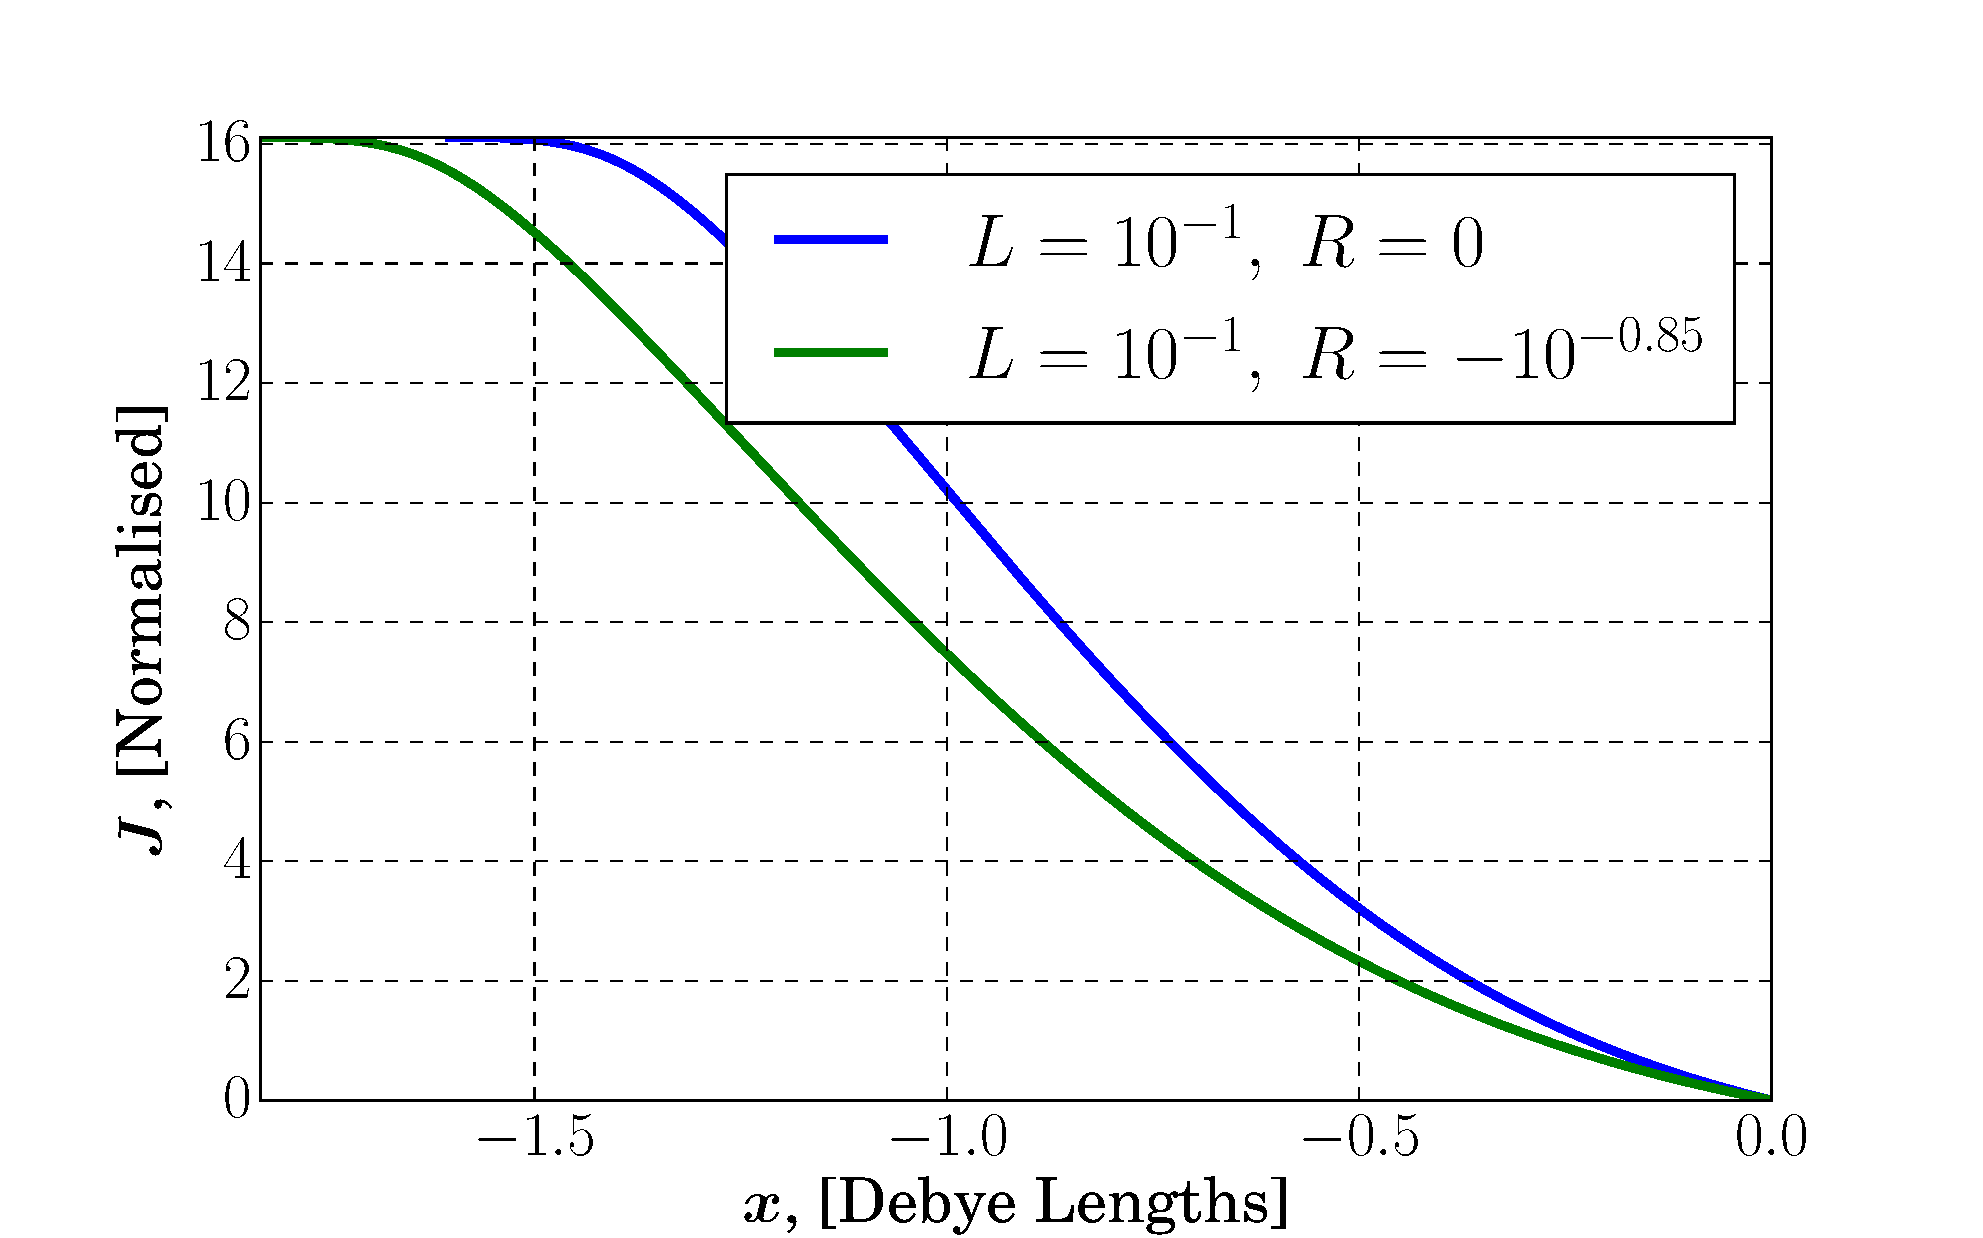
\includegraphics[width=0.3\linewidth]{0_-1l.eps}
			~
			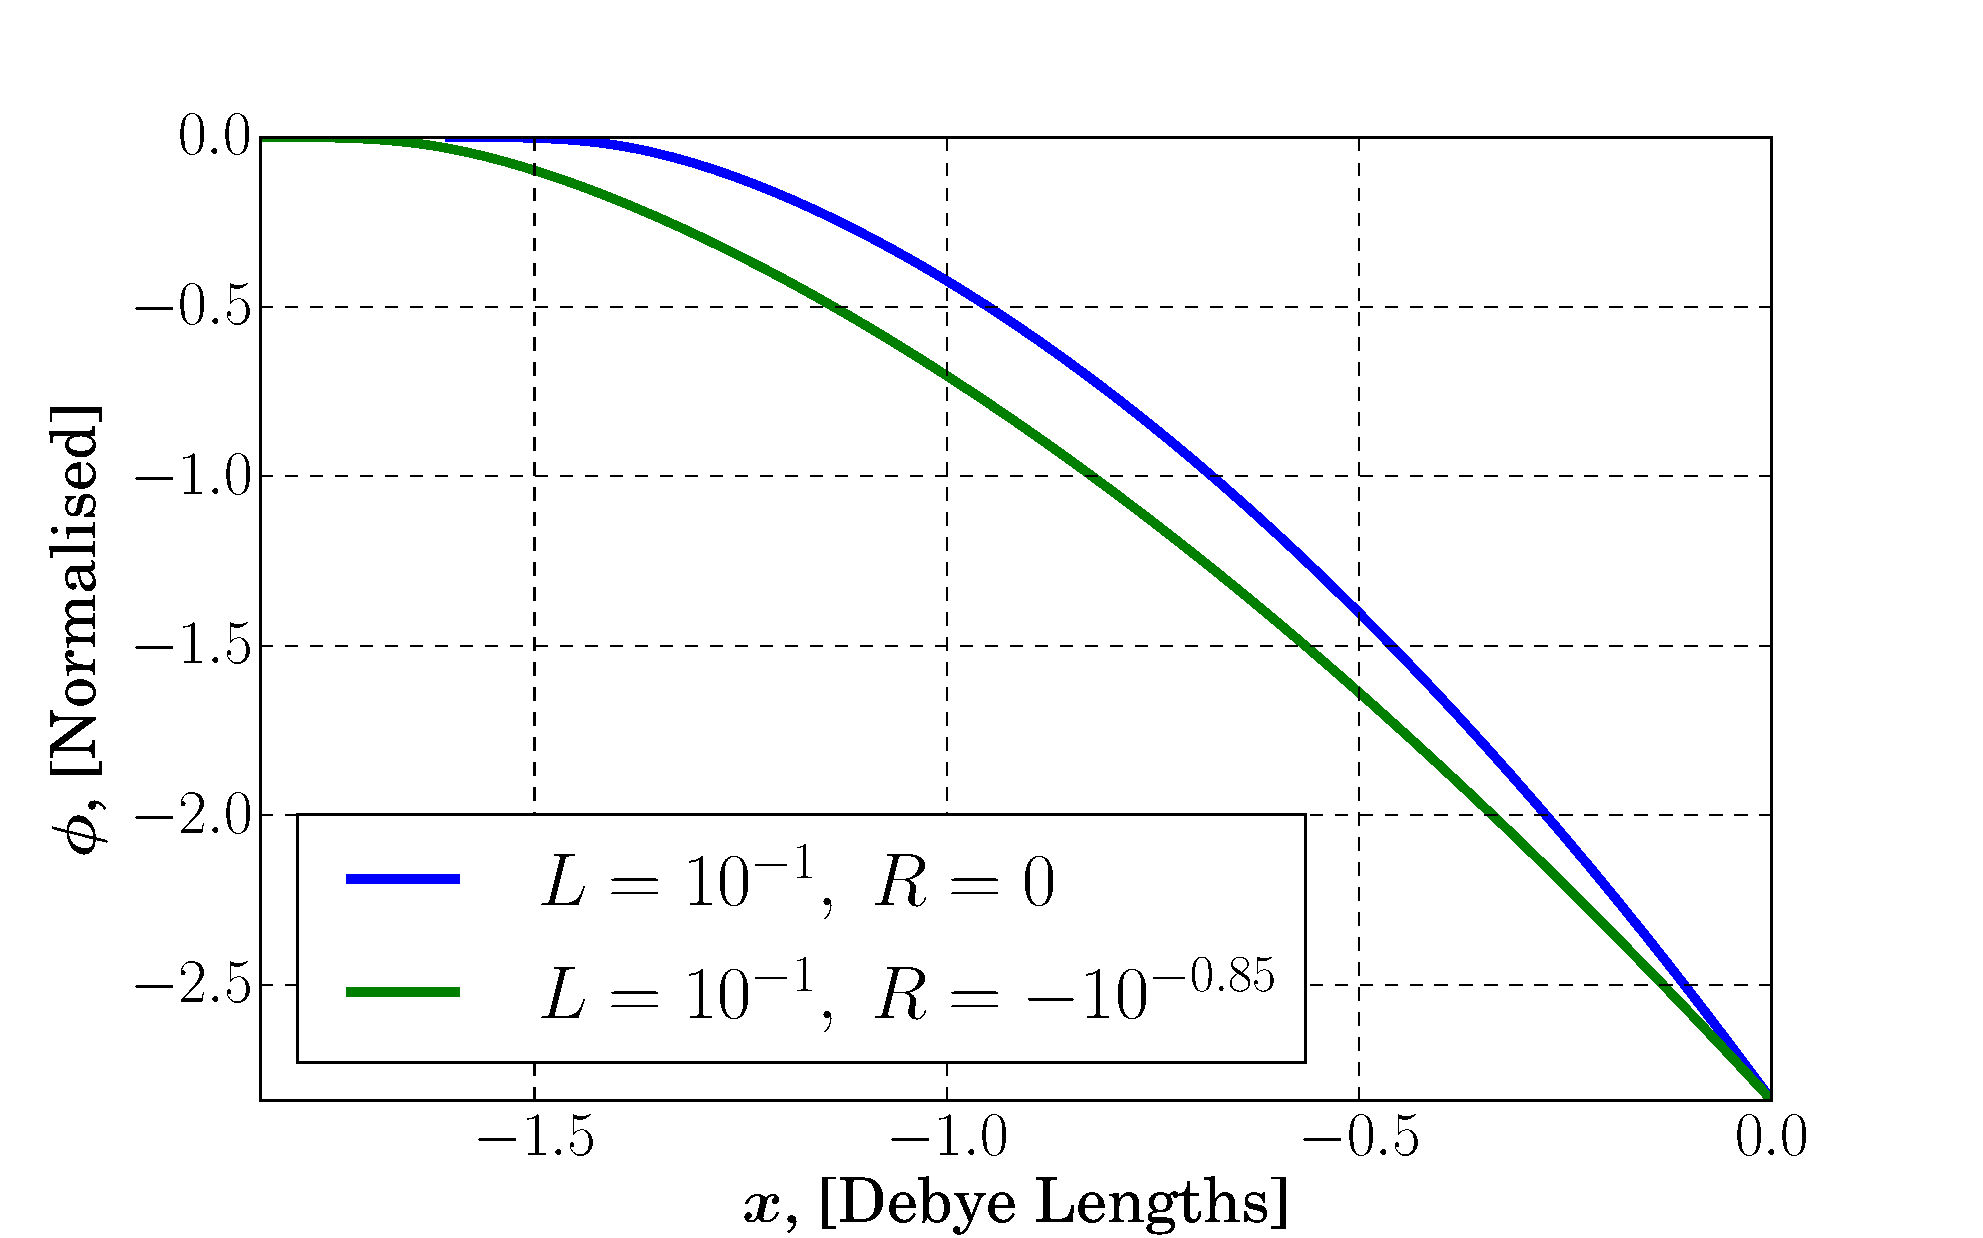
\includegraphics[width=0.3\linewidth]{1_-1l.eps}
			~
			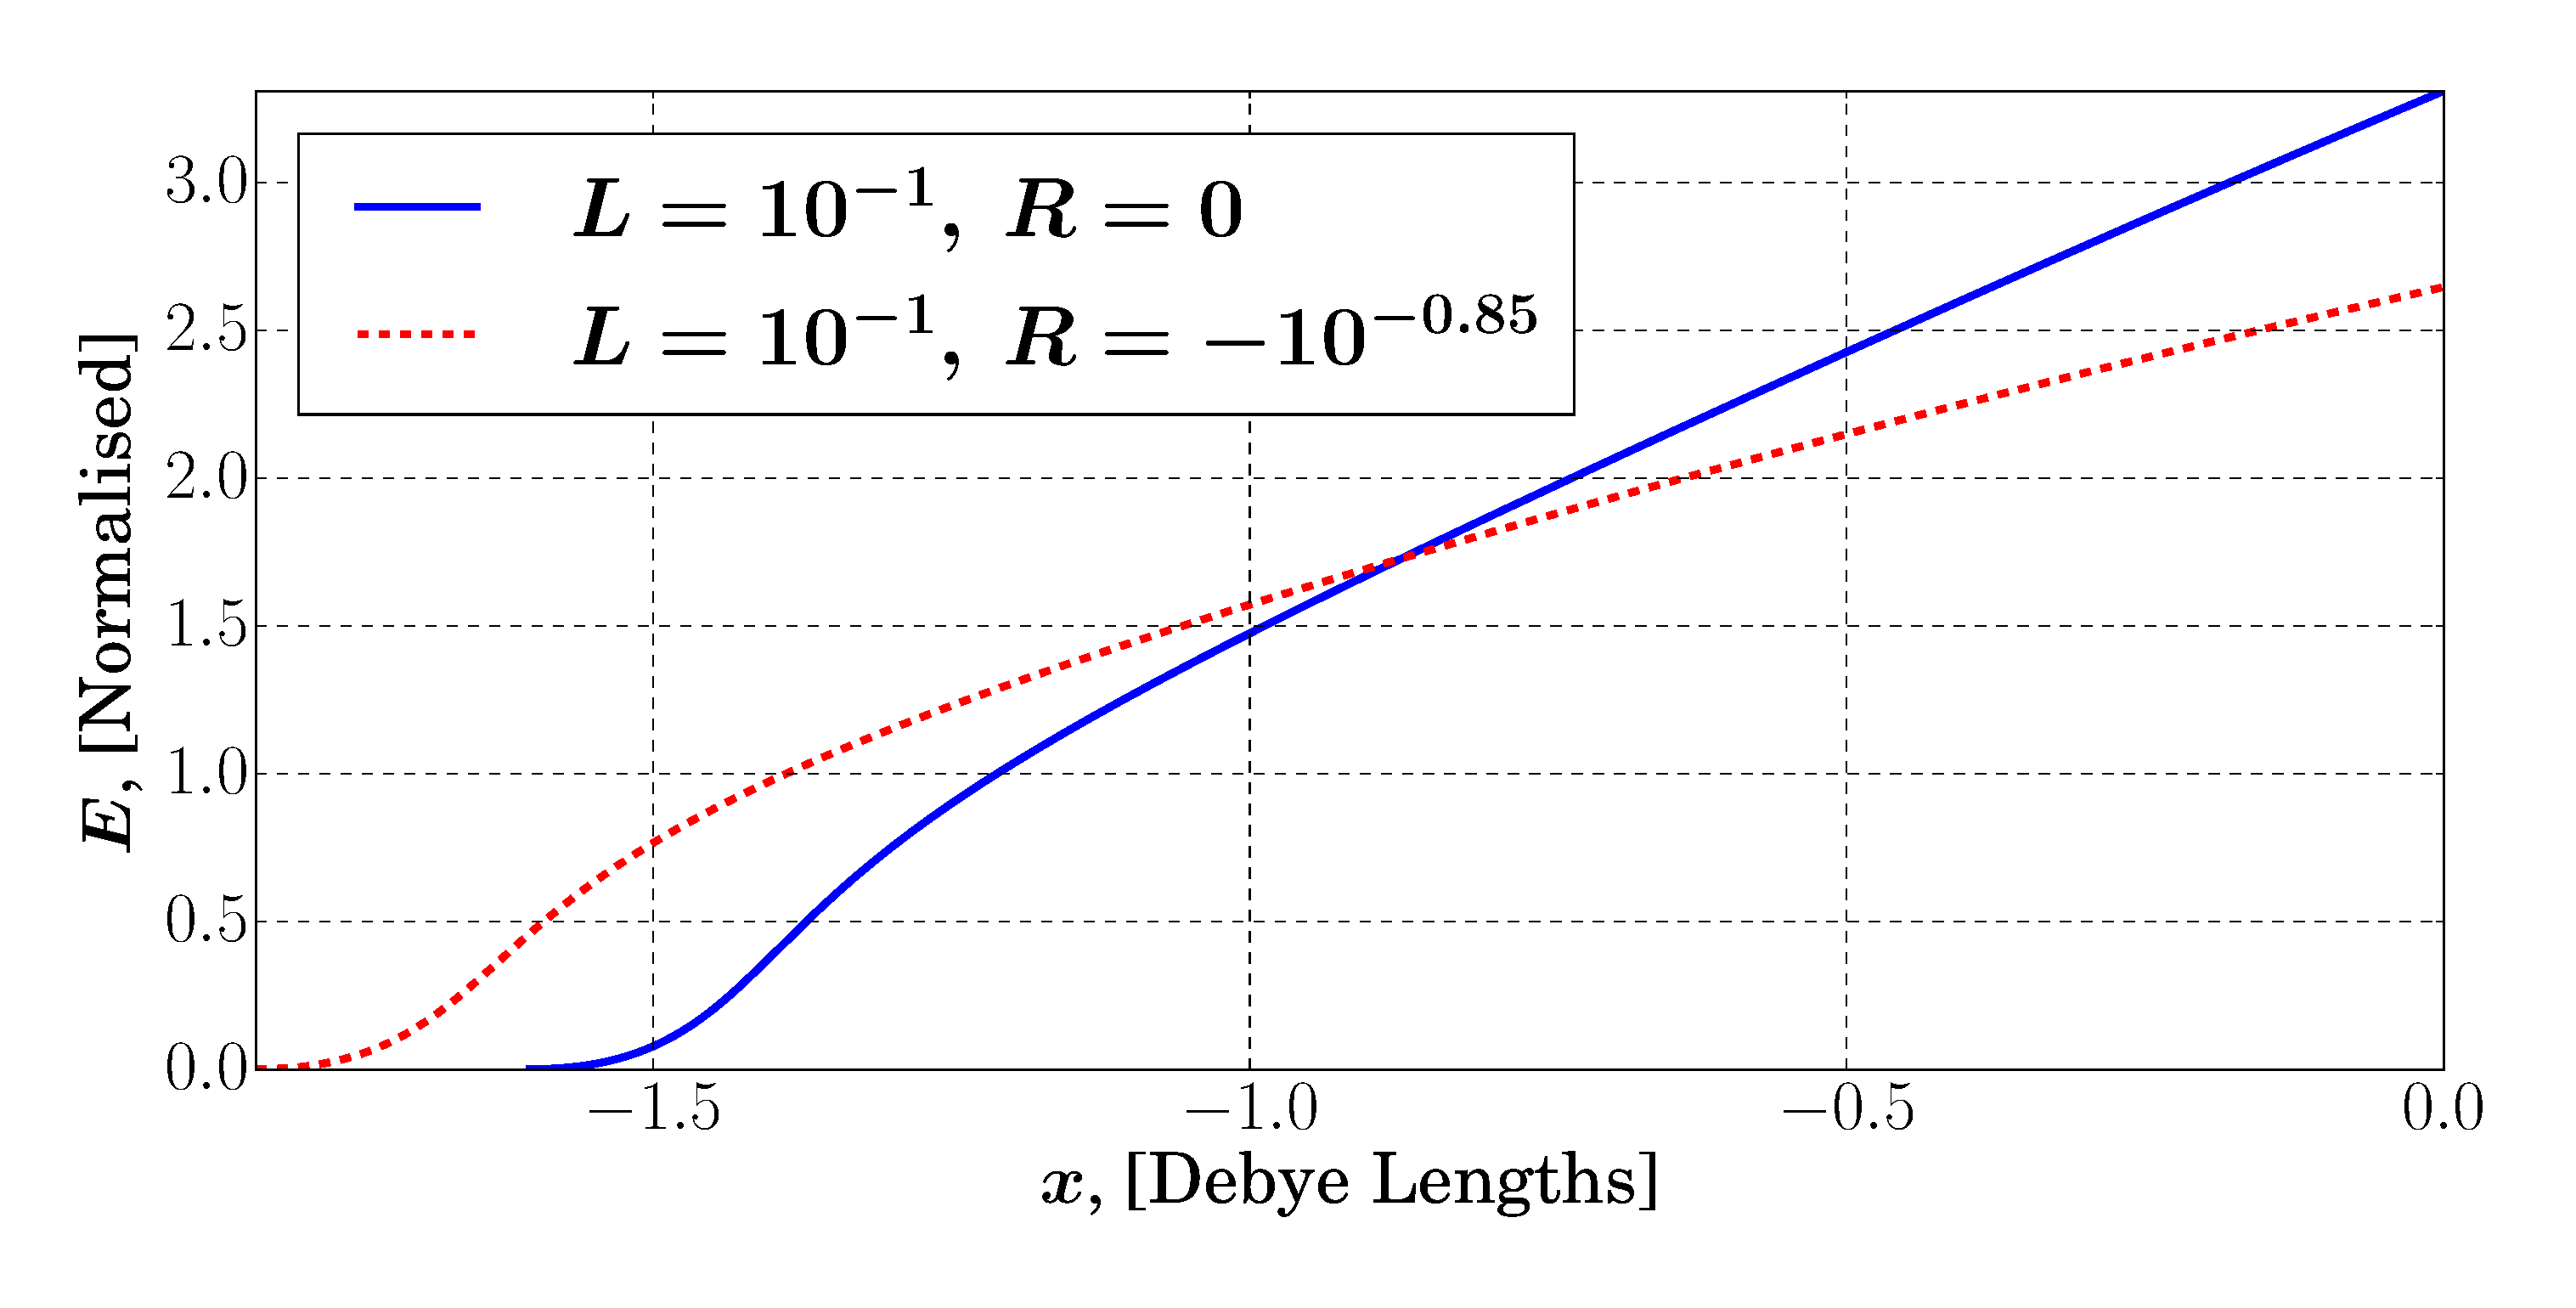
\includegraphics[width=0.3\linewidth]{2_-1l.eps}
			
			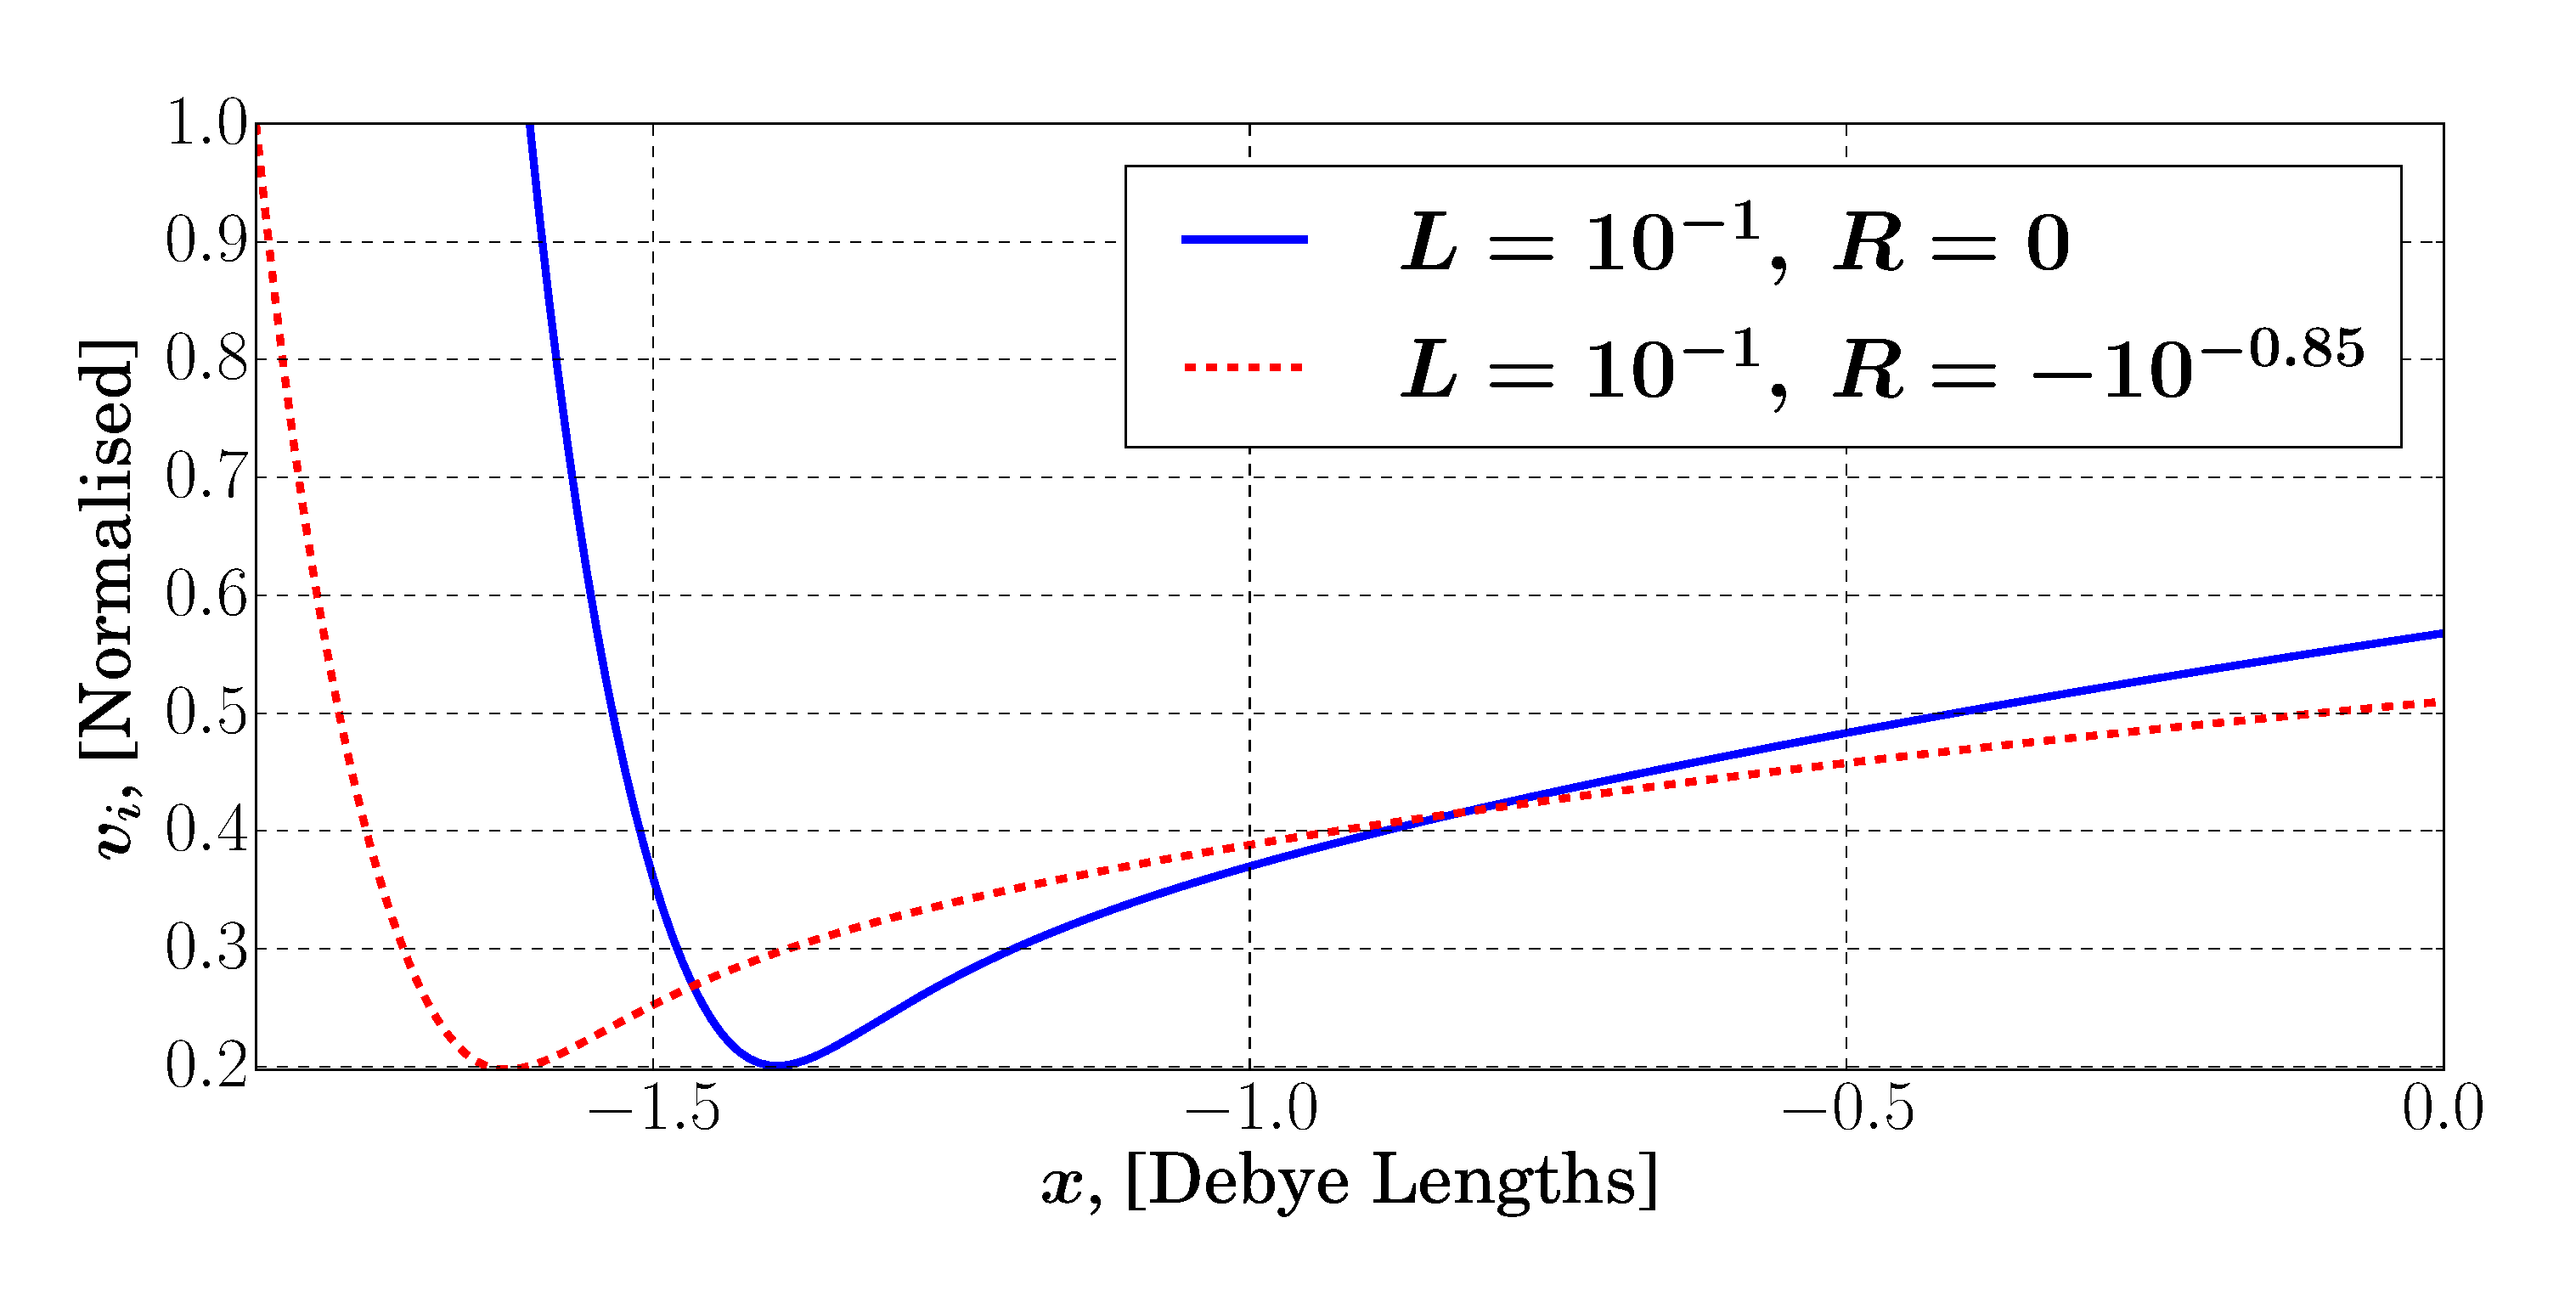
\includegraphics[width=0.3\linewidth]{3_-1l.eps}
			~
			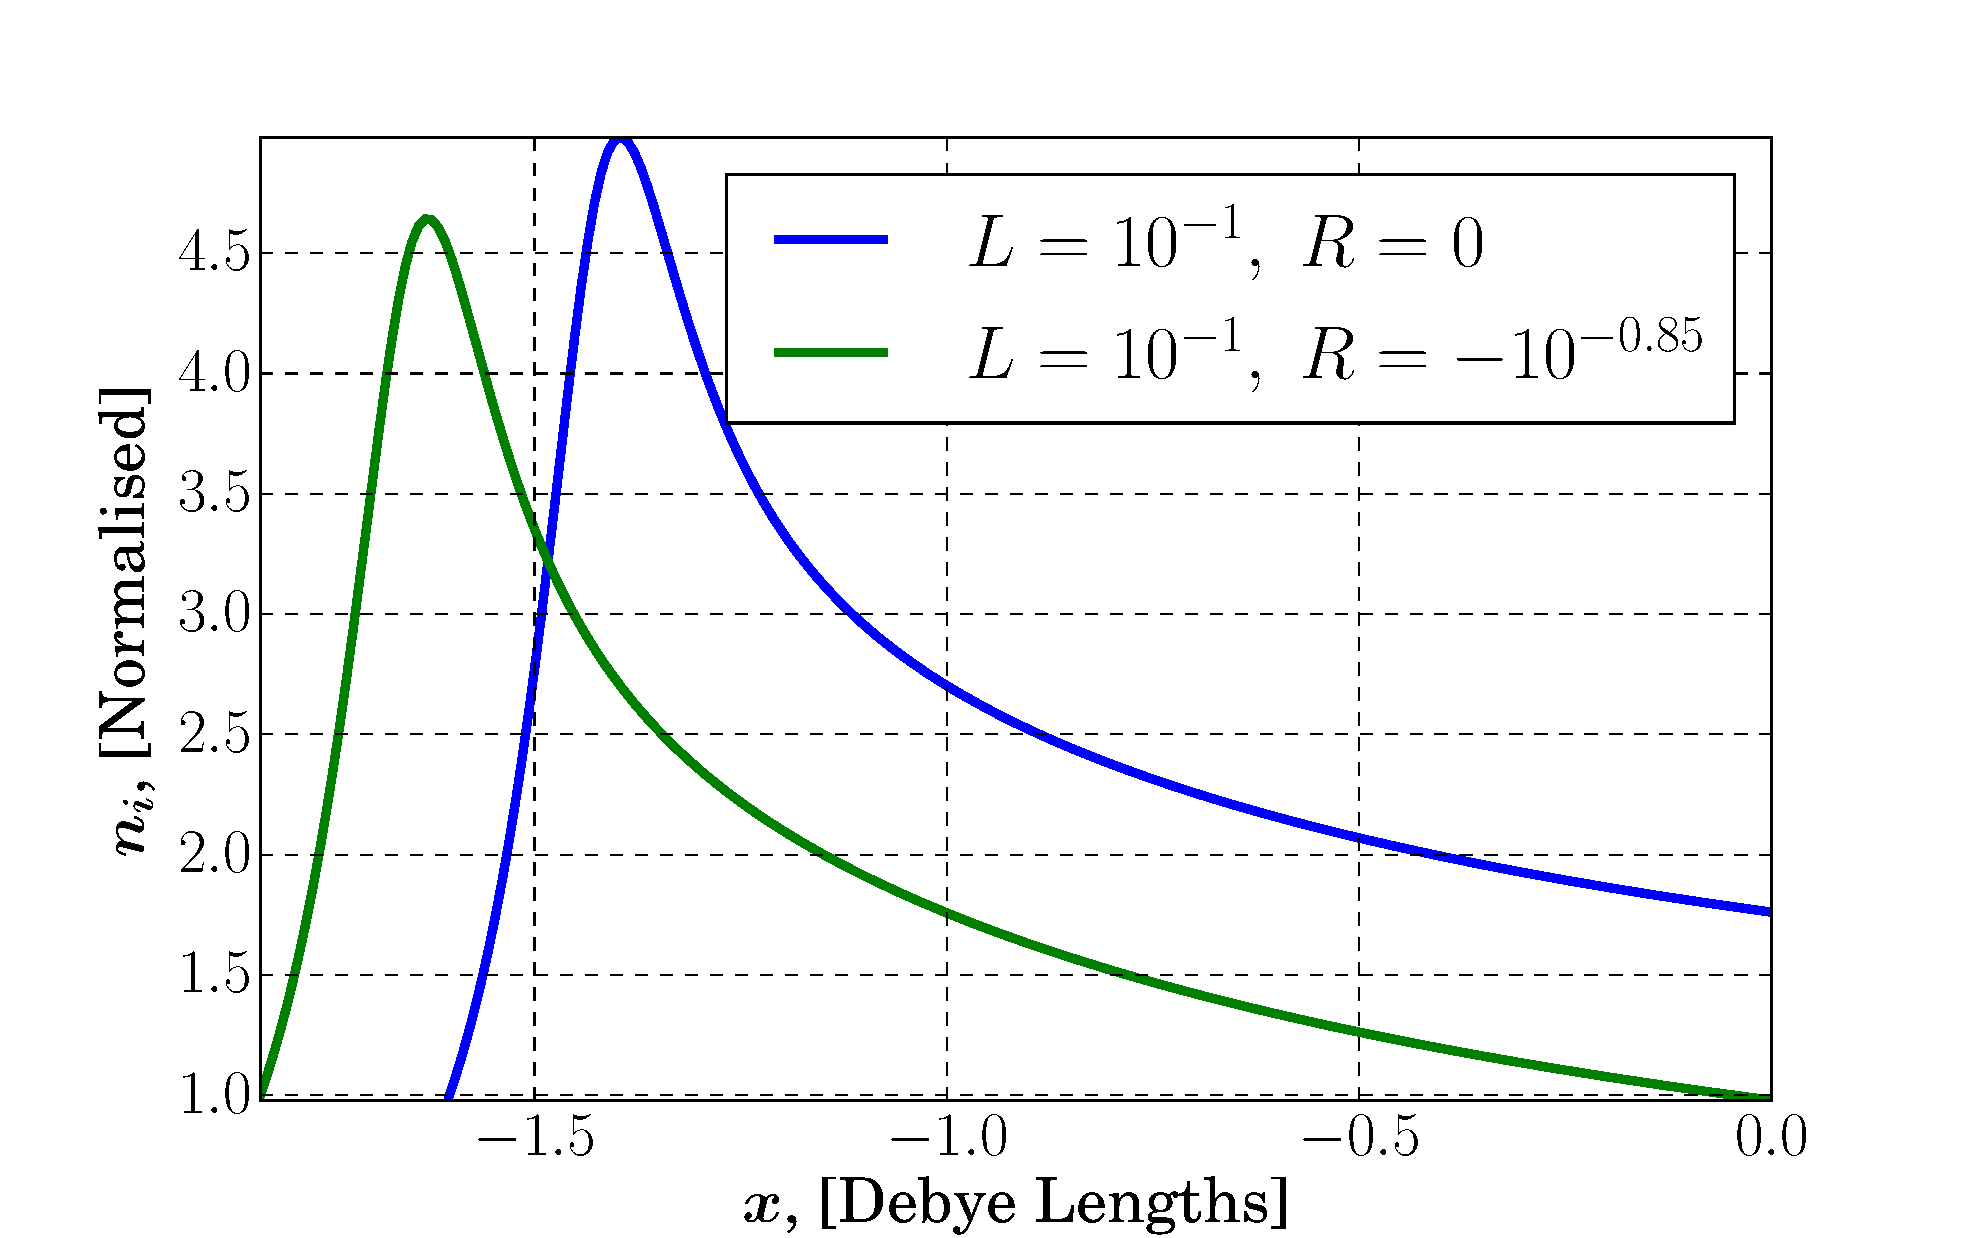
\includegraphics[width=0.3\linewidth]{4_-1l.eps}
			~
			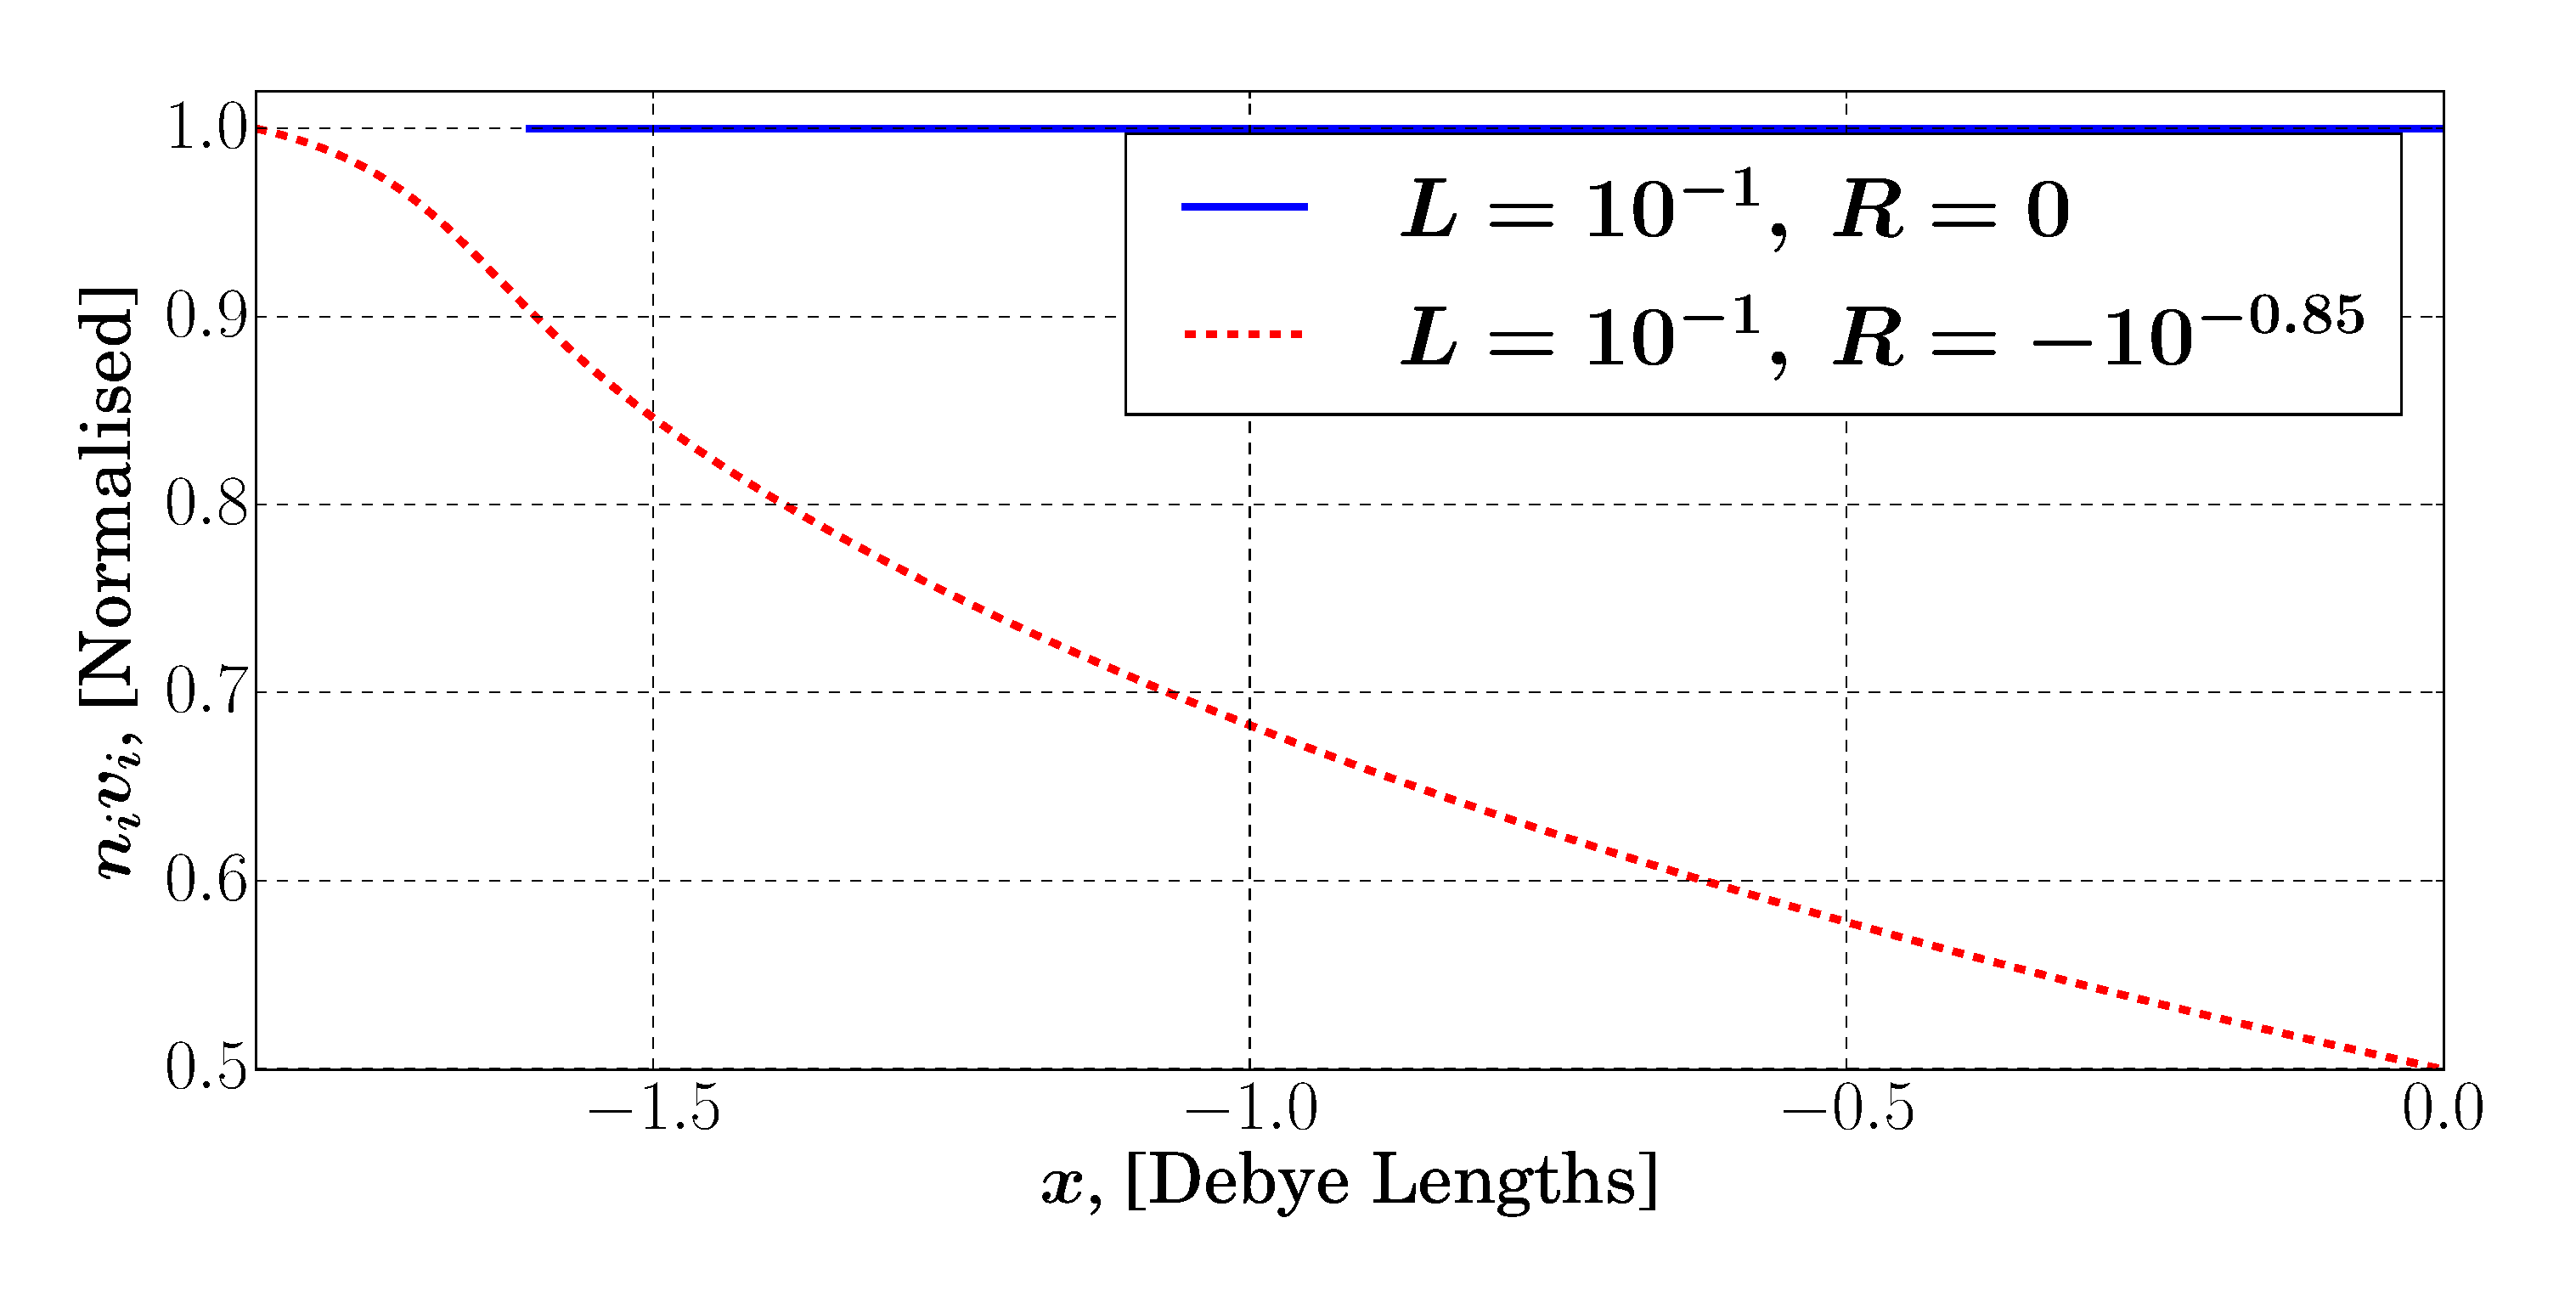
\includegraphics[width=0.3\linewidth]{6_-1l.eps}
			\caption{$ L = 10^{-1},~ R = -10^{-0.85}~\textrm{(Green)}~,~ R = 0~\textrm{(Blue)} $.}
			\label{sf:rslta}
		\end{subfigure}
		
		\begin{subfigure}[t]{\linewidth}
			\centering
			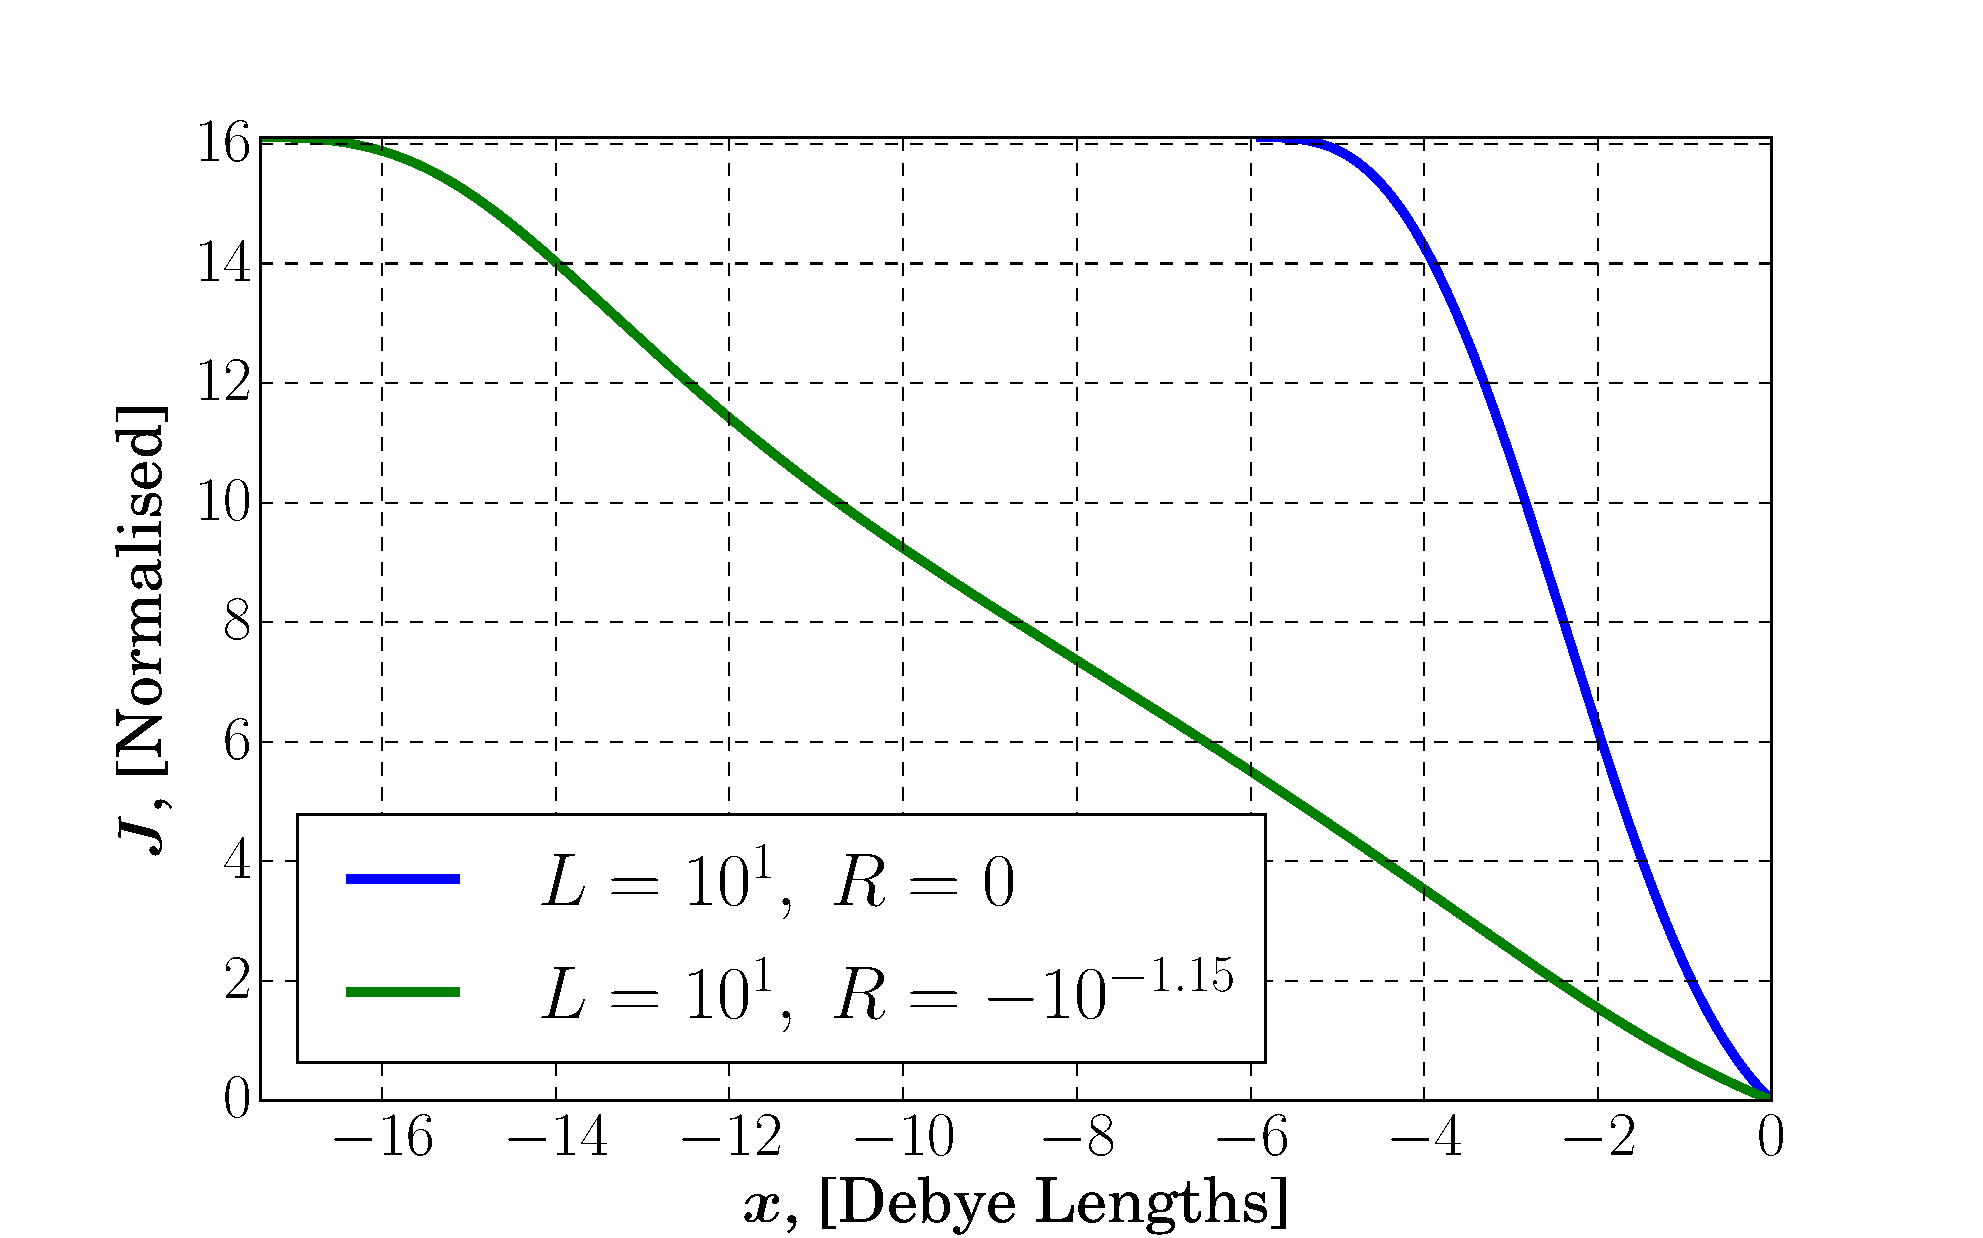
\includegraphics[width=0.3\linewidth]{0_1l.eps}
			~
			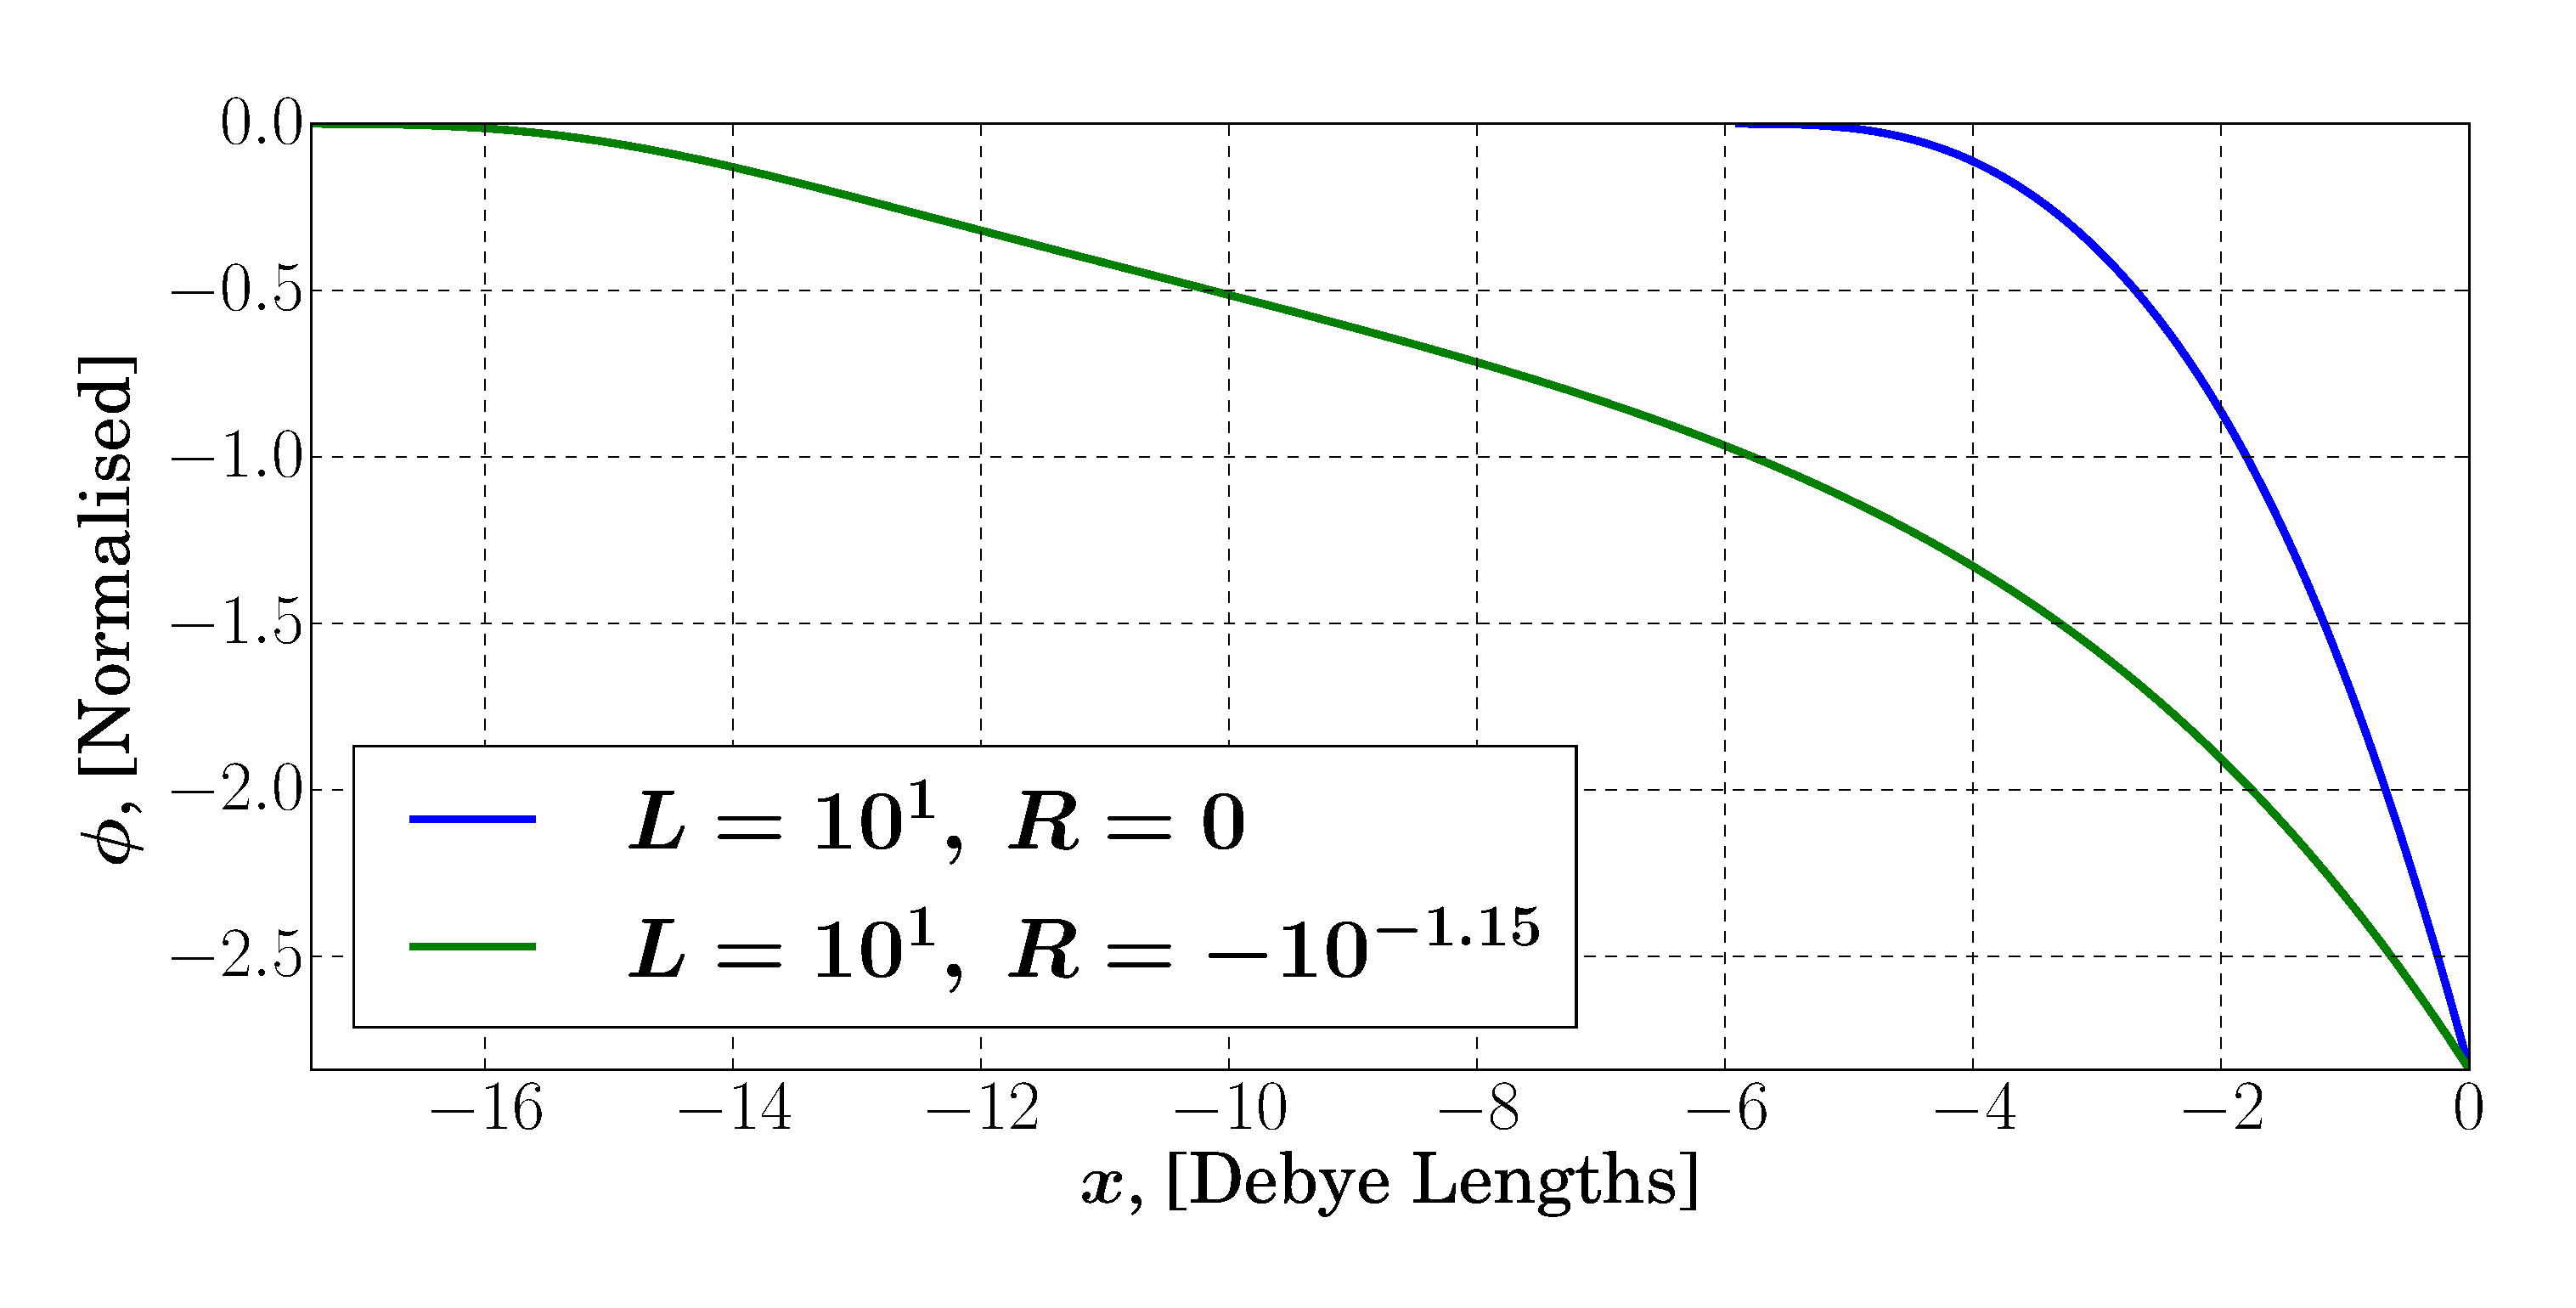
\includegraphics[width=0.3\linewidth]{1_1l.eps}
			~
			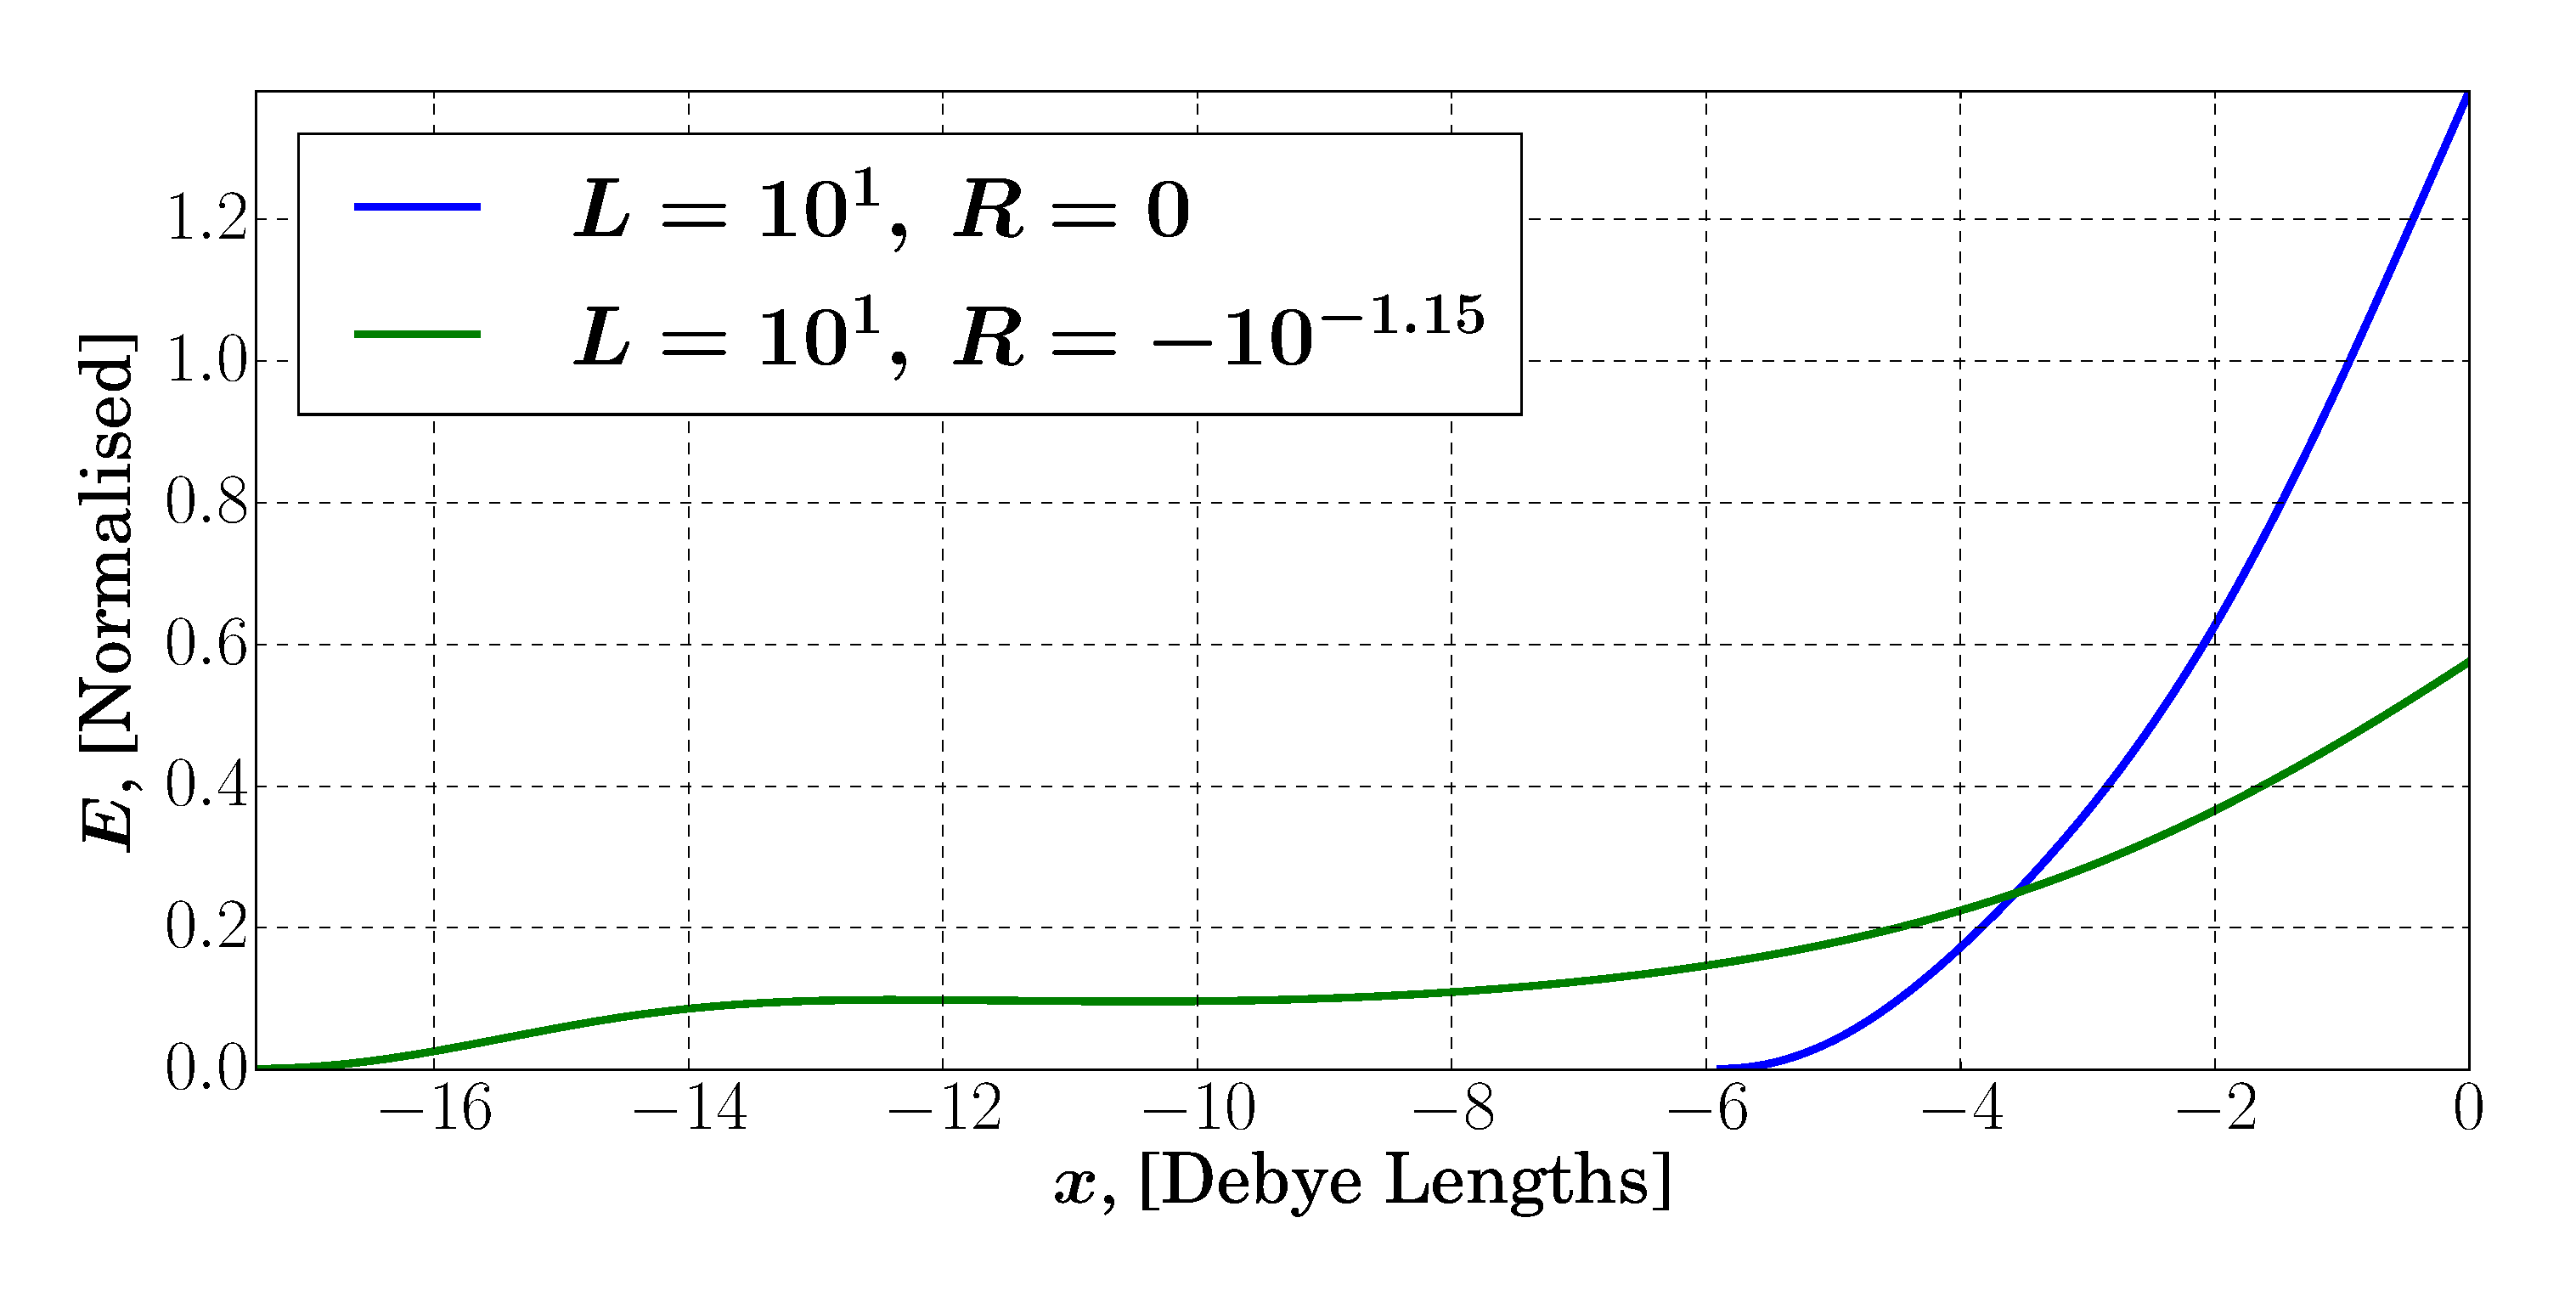
\includegraphics[width=0.3\linewidth]{2_1l.eps}
			
			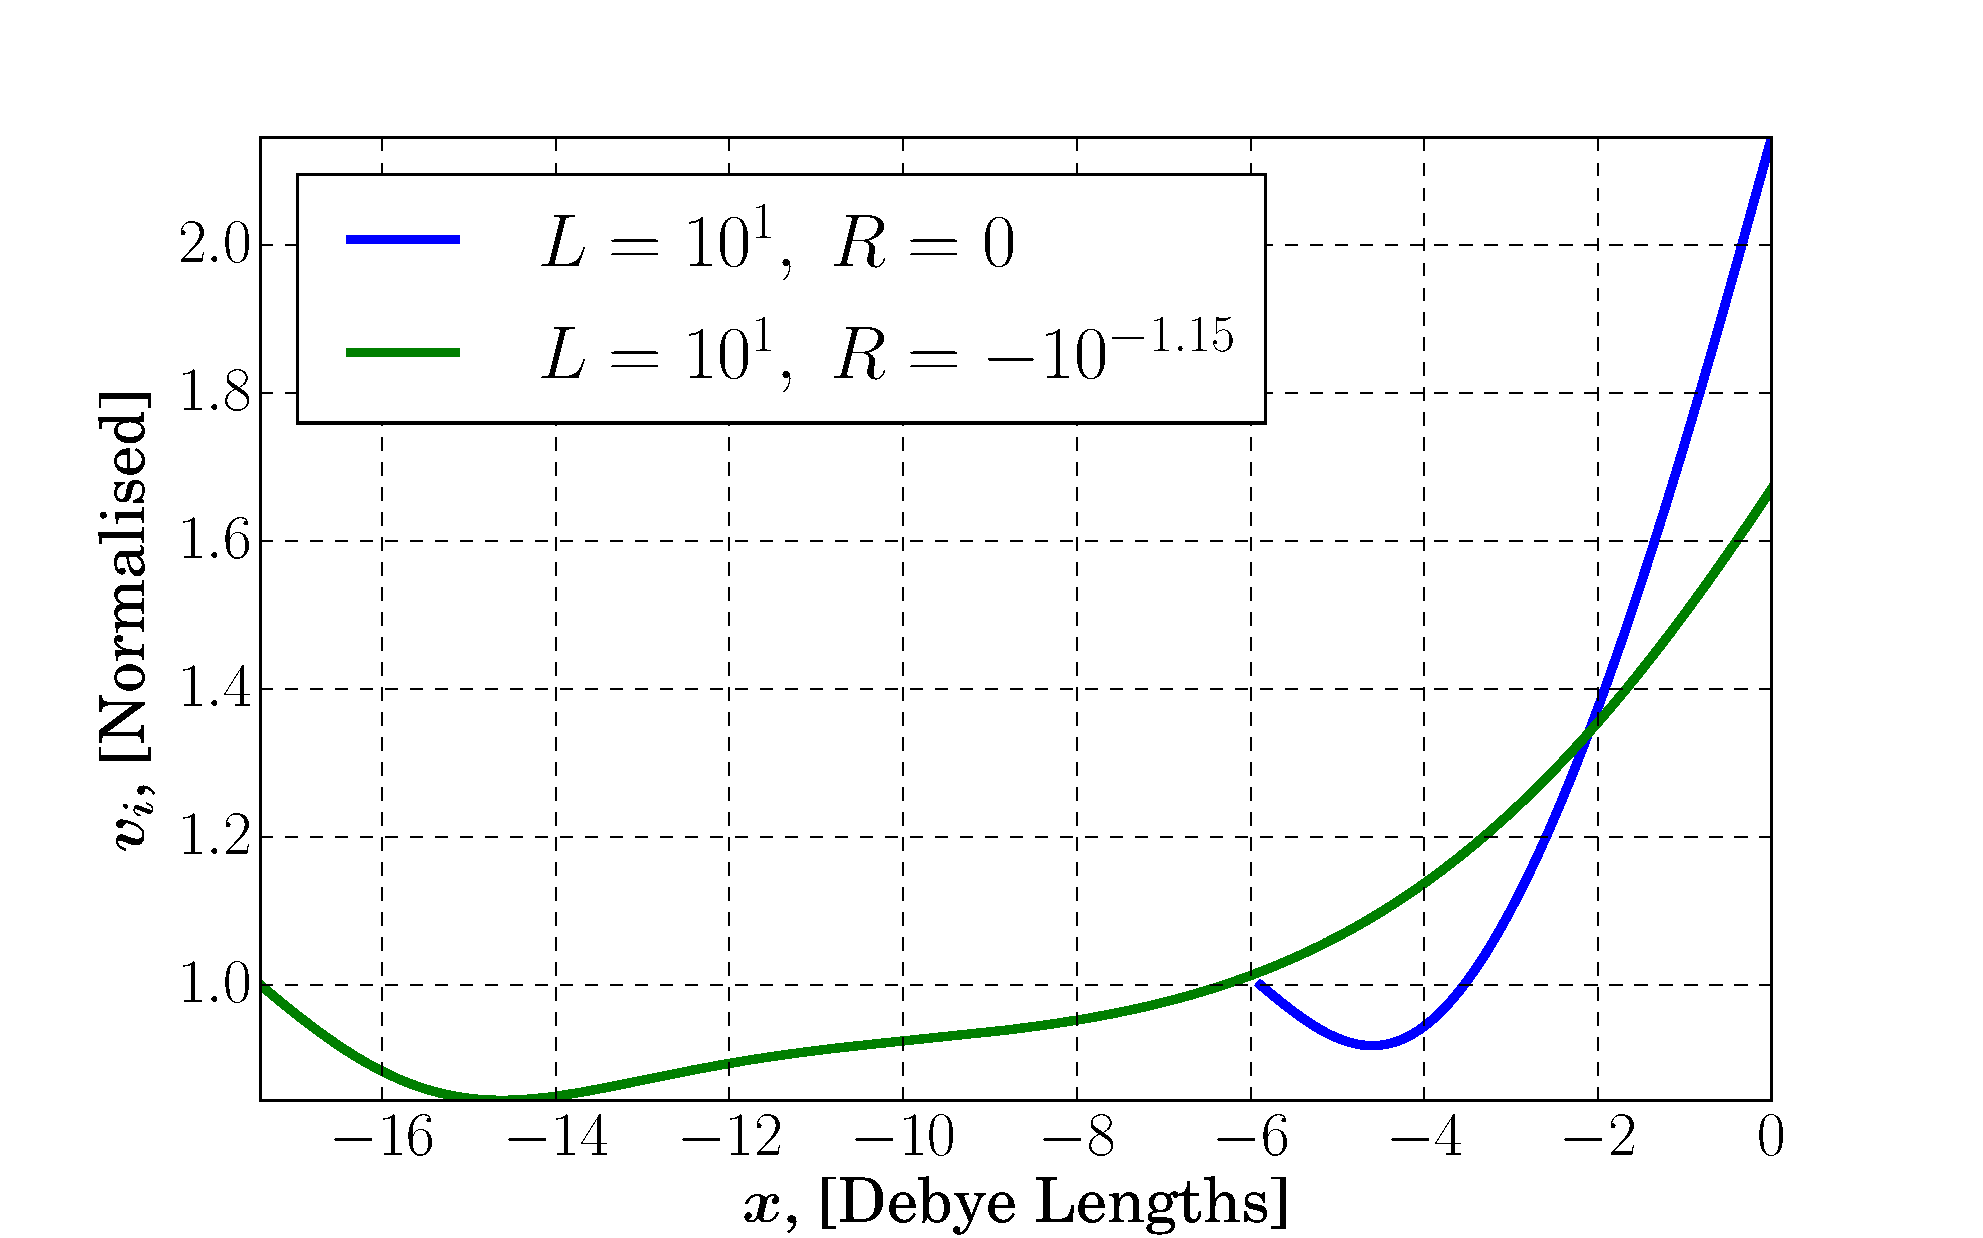
\includegraphics[width=0.3\linewidth]{3_1l.eps}
			~
			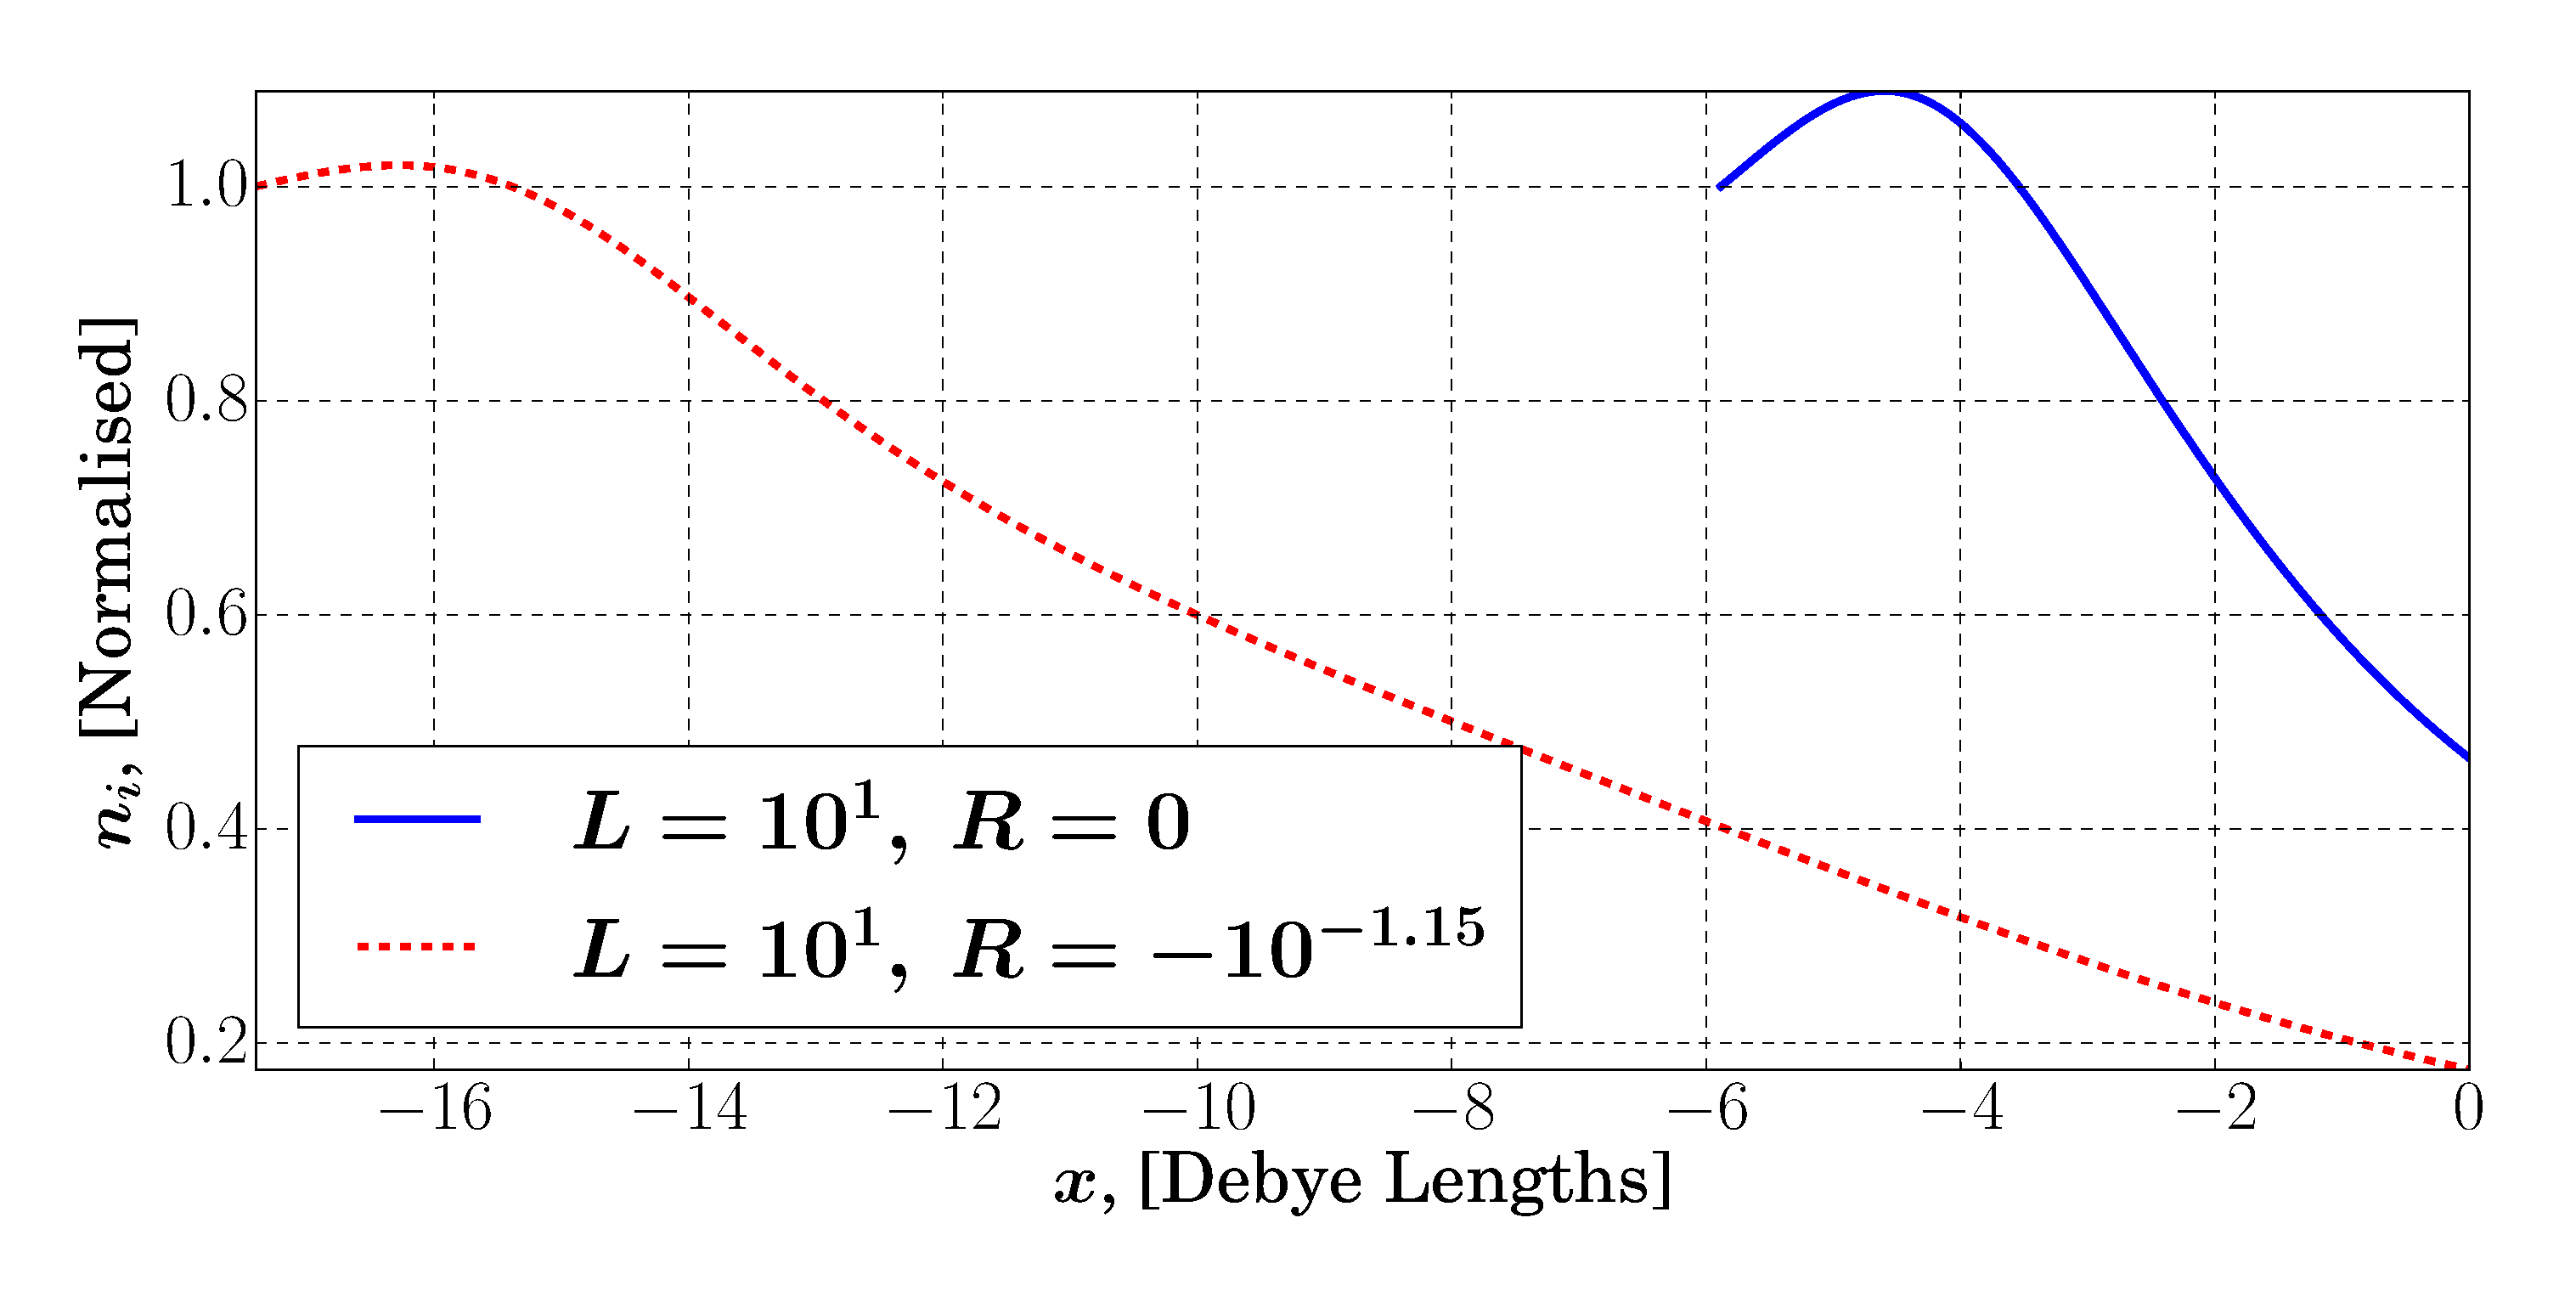
\includegraphics[width=0.3\linewidth]{4_1l.eps}
			~
			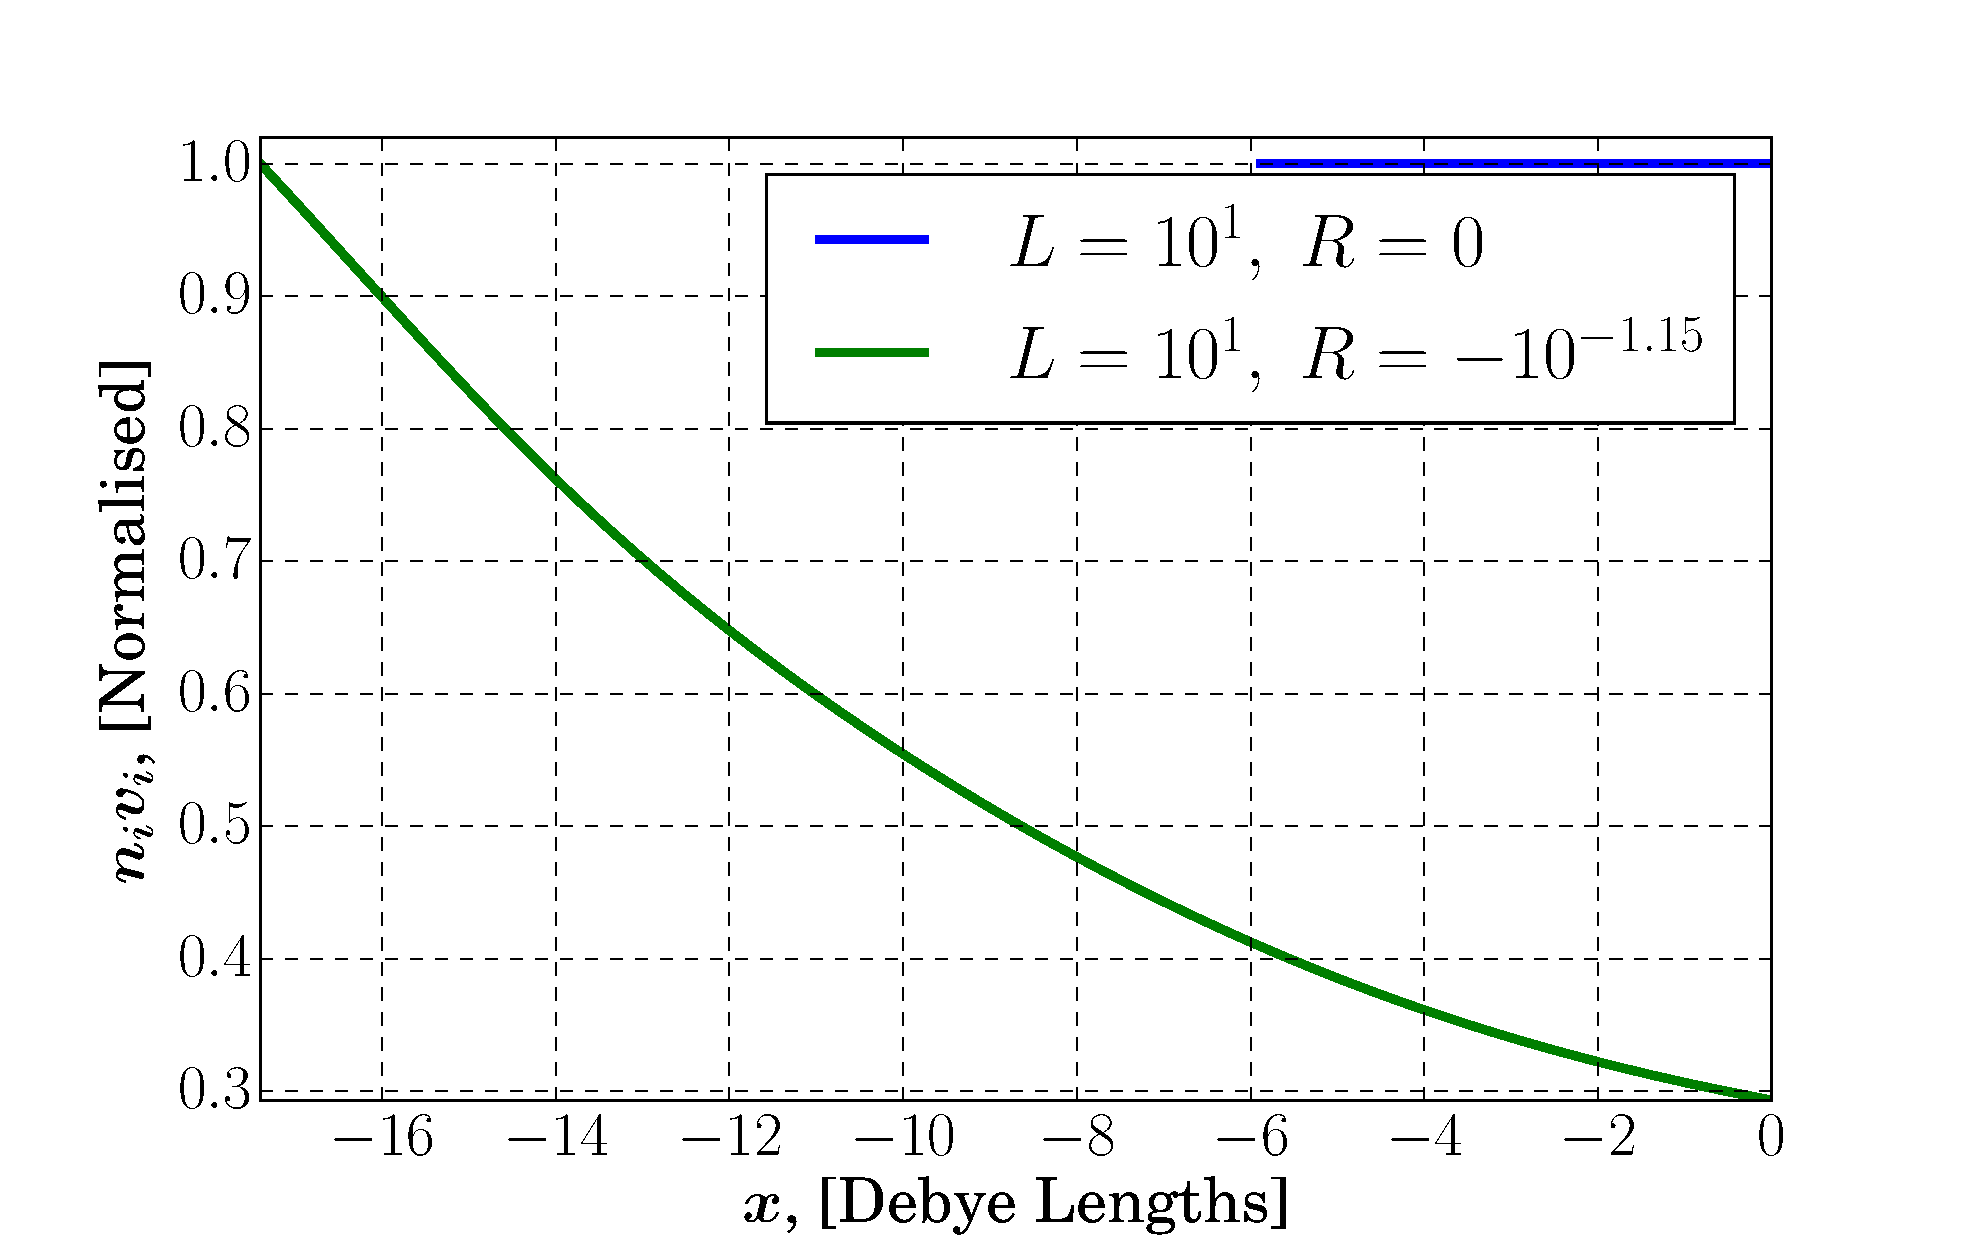
\includegraphics[width=0.3\linewidth]{6_1l.eps}
			\caption{$ L = 10,~ R = -10^{-1.15}~\textrm{(Green)}~,~ R = 0~\textrm{(Blue)} $.}
			\label{sf:rsltb}
		\end{subfigure}
		\caption{Left to right, top to bottom: current, electrostatic potential, electric field, and ion velocity, density and continuity. All as a function of distance from the wall at $x=0$.}
		\label{f:rslt}
	\end{figure*}
	
	It was found that in order for the Debye sheath to remain stable, the magnitude of the normalised recombination constant should approximately satisfy the inequality,
	\begin{align}
		L \times 10^{x} > |R| \times 10^{-|x+0.15|}.\label{e:rl}
	\end{align}
	Else the rate at which ions are lost through recombination is so great that the solutions for \cref{e:sheath} are non-smooth, indicating the sheath becomes unstable and breaks down.
	
	From \cref{sf:rslta} that at short collision lengths and comparable recombination rates, the overall dynamics of the system don't change. Aside from the ion continuity equation, the system looks very similar for both values of $R$---indicating the dominant behaviour is the collision length as opposed to the recombination rate. Conversely, from \cref{sf:rsltb}, we see a much greater difference between systems. Not only does the sheath grow to almost three times the size of the unmodified case, but the profile of every quantity changes significantly. In this regime, the recombination becomes much more important. 
	
	\section{Discussion}\label{s:discussion}
	In order to explain our choice of parameters we turn to \cref{se:s3}. Firstly we note that,
	\begin{subequations}
		\begin{align}
			\lim\limits_{L \to \infty} \difx{v_{i}} &= \dfrac{E}{v_{i}}\\
			\lim\limits_{L \to \infty} \int\limits_{v_{s}}^{v_{i}} v_{i} \mathrm{d}v_{i} &= \int E \mathrm{d}x\\
			\lim\limits_{L \to \infty} v_{i} &= \sqrt{v_{s}^{2} - 2\phi}.\label{se:vi}
		\end{align}
	\end{subequations}
	Meaning that \cref{se:s3} asymptotically approaches the value of the unmodified model. Furthermore, if $L \to 0 \Rightarrow \difx{v_{i}} \to \infty$. Therefore we must keep $L$ reasonably small if we want avoid asymptotic behaviour to the unmodified model, and reasonably big if we want to keep our solutions smooth.
	
	Secondly we realise that,
	\begin{subequations}
		\begin{align}
			\lim\limits_{R \to 0} \difx{n_{i}} &= -\dfrac{n_{i}}{v_{i}} \difx{v_{i}} \\
			\lim\limits_{R \to 0} \int\limits_{1}^{n_{i}}\dfrac{\mathrm{d} n_{i}}{n_{i}} &= -\int\limits_{v_{s}}^{v_{i}}\dfrac{\mathrm{d} v_{i}}{v_{i}}\\
			\lim\limits_{R \to 0} n_{i}v_{i} &= v_{s},
		\end{align}
	\end{subequations}
	is the ion continuity equation (a constant value). So we must keep $|R| > 0$ if we want to compare the modified model to the case with no recombination. 
	
	At the same time we know from \cref{se:s4} that if,
	\begin{subequations}
		\begin{align}
			\left|R - \difx{v_{i}}\right| &\ggg 0 \\
			\textrm{ assuming: } R + \dfrac{v_{i}}{L} &\gg \dfrac{E}{v_{i}} \nonumber \\
			\left|R + \dfrac{v_{i}}{L}\right| &\ggg 0
		\end{align}
	\end{subequations}
	the solution to \cref{se:s4} would be non-smooth. This analysis prompted our choice of parameters. The definition of \cref{e:rl} was obtained so that the solutions across $L \in [10^{-7}, 10^{7}]$ remained smooth yet sufficiently different from the case where $R = 0$.
	
	With this information, our observations---and choice to include only two values of $L$---can be fully explained. Looking at \cref{se:s3} we realise that the extent to which $R$ affects the system depends on the magnitude of $L$. As $L \to 0$, the effect of $R$ will be minimised because $L^{-1} \to \infty$ and thus dominate in \cref{se:s4}. On the other hand, as $L$ grows, $R$ will begin to have more of an effect on \cref{se:s4} until $L$ is so large that \cref{se:s3} starts converging to \cref{se:vi}. At which point, given \cref{e:rl} and $\dfrac{E}{v_{i}} \gg R$, $R$ will once again stop having a noticeable effect on \cref{se:s4}. Thus by choosing $L = \left\{10^{-1}, 10\right\}$, we observe appreciable differences between scenarios, something which is not the case for other values.
	\begin{comment}
	\begin{itemize}
		\item Summarises main findings
		\item Discussion of the implications of your result
		\item Relates results to literature and introduction
		\item Guidline length $ \dfrac{1}{2} \to 1 $ page
		\item 20\%
	\end{itemize}
	content...
	\end{comment}
	
	\section{References}
	\bibliography{dcg513}
	%Use academic books and articles as references, 20\%.
	\begin{comment}
	\section{Structure and presentation}
	\begin{itemize}
		\item Good use of English
		\item Clear, legible layout
		\item Each section is relevant to the next, and sections refer to each other where appropriate
		\item 20\%
	\end{itemize}
	\end{comment}
	
\end{document}